% ---------------------------------------------------------------------------
%  Every number below is produced by scripts/ and stored in results/tables/.
%  Compile: pdflatex paper.tex  (twice, for cross-references)
% ---------------------------------------------------------------------------
\documentclass[11pt,a4paper]{article}

\usepackage[margin=2.5cm]{geometry}
\usepackage{amsmath,amssymb}
% Times-like text and matching maths. The LaTeX default (Computer Modern)
% is universal in mathematics and rare in epidemiology, which is the
% readership this is aimed at.
\usepackage{newtxtext,newtxmath}
\usepackage{graphicx}
\usepackage{booktabs}
\usepackage[hidelinks]{hyperref}
% Let long URLs break across lines; the repository URL overflows otherwise.
\usepackage{xurl}

\graphicspath{{../results/figures/}}

\title{\bfseries How much of the evidence for climate-driven dengue\\
transmission survives the analyst?\\
\large A multiverse analysis of 221 outbreaks in 33 countries}

\author{Amna Dilber\\
\small Independent researcher, Lahore, Pakistan\\
\small \texttt{amnadilber.bi@gmail.com}\\
\small ORCID: \href{https://orcid.org/0009-0008-5684-4516}{0009-0008-5684-4516}}

\date{Draft, \today}

\begin{document}
\maketitle

\begin{abstract}
\noindent
Compartmental models fitted to surveillance data are routinely used to test
whether dengue transmission is climate-driven, and reviews explain their
conflicting findings by appealing to local context. We fit every usable outbreak
in a global surveillance compilation under all 144 combinations of six analysis
choices that published models rarely state, so that no choice varies with the
setting because none varies at all: 33{,}152 fits, of which the 221 outbreaks in
33 countries completing every combination are analysed.

\textbf{Roughly three-quarters of the variation in whether climate forcing is
endorsed lies between analyses of the same outbreak, not between outbreaks}
(76.5\%; 95\% CI 72.6--81.1 resampling whole countries). Partitioned three ways
the largest term is neither: \textbf{61\%} is an outbreak-by-analysis
interaction, against 16\% for the analysis itself, so no standardised convention
can reach it and a specification curve, which displays the main effect, cannot
show it. Adding climate covariates moves estimated $R_0$ the same way, its
interaction share rising from 23\% to 69\%.

The intervals do not keep their promise. A nominal 95\% interval contains the
true transmission coefficient \textbf{78\%} of the time and the true rainfall
coefficient \textbf{71\%}, falling to \textbf{42\%} when the epidemic is a
sum of two
asynchronous ones, as these data demonstrably are. Combining \textbf{eight}
analyses by Rubin's rules restores nominal coverage at 1.5--2.2 times the width,
reaching 90\% rather than 95\% under structural mis-specification.

Applying our own rule gives a clear verdict for 137 of 221 outbreaks,
\textbf{86\% of which support climate forcing}, and the three-way partition of
the real data matches simulated outbreaks containing a real effect rather than
simulated outbreaks containing none. The claim is not that the effect is absent,
but that in 38\% of outbreaks a single season cannot settle the question.
\end{abstract}

% ===========================================================================
\section{Introduction}
% ===========================================================================

Whether dengue transmission is driven by climate is asked repeatedly of
surveillance data, and the answer feeds early-warning systems, attribution
studies and control policy. The usual method is to fit a transmission model with
and without climate covariates and compare them by an information criterion.

Such an analysis requires decisions that the model itself does not determine. A
distribution must be chosen for the observation error. A functional form must be
chosen for the temperature response. Rainfall must be lagged by some number of
weeks: a lag with a mechanistic basis and no agreed value, since both drought
and extreme rainfall raise dengue risk at different delays~\cite{lowe2021}. Some portion of the series must be set aside for validation, or none. None
of these is a hypothesis about dengue; each is a convention, and published papers
rarely state why one was preferred over another.

A systematic review of 99 dengue prediction models from 64 studies found that
``[t]he reporting of methodology and model performance measures were inadequate
in many of the existing prediction models''~\cite{review2023}. The field is aware of the
problem. What has not been quantified is its consequence: how often the reported
conclusion would have differed had the analyst chosen otherwise.

We measure this directly. Every usable dengue outbreak in a global surveillance
compilation (221 of them, in 33 countries) is fitted under a full factorial
of six such choices, 144 combinations and 33{,}152 fits, so that no analytical
choice varies with the setting because none varies at all. Four things follow.

\begin{enumerate}
\item \textbf{The disagreement in this literature is mostly not geographic.}
      Roughly three-quarters of the variation in whether an outbreak is judged
      climate-driven lies between analyses of the same outbreak rather than
      between outbreaks (Section~\ref{sec:decomposition}). Everything that differs
      between epidemics competes for the remaining quarter, which bounds what any
      contextual explanation can achieve, and the specific contextual
      explanation on offer does not reproduce here. Partitioning three ways, the
      largest term is an outbreak-by-analysis interaction at 61\%, four times the
      main effect of the analysis: the disagreement is not a ranking of methods
      that a house style could settle.
\item \textbf{The cost falls on the number the field reports.} Under a constant
      model, 72\% of the variation in estimated $R_0$ lies between outbreaks,
      which is what an estimate is for. Adding climate covariates inverts that:
      80\% or more of the variation is then between analyses of the same outbreak
      (Section~\ref{sec:r0}).
\item \textbf{The intervals do not keep their promise.} A nominal 95\% interval
      contains the true transmission coefficient 78\% of the time, and the true
      rainfall coefficient 71\%, falling to 42\% when the epidemic is a sum of two
      asynchronous ones, which these data demonstrably are
      (Section~\ref{sec:coverage}).
\item \textbf{An interval that does keep it, validated against a known truth and
      cheap enough to use.} Combining the analyses by Rubin's rules restores
      nominal coverage at 1.5 to 2.2 times the width, and \textbf{eight analyses
      are enough}: four already reach nominal. It is an improvement rather than
      a cure: under structural mis-specification it falls to 90\%, and we report
      that rather than the headline alone.
\end{enumerate}

The diagnosis is therefore accompanied by an instrument, and the instrument has
been tested where it fails as well as where it works.

\paragraph{Relation to multiverse and specification-curve analysis.} The design
is a multiverse analysis in the sense of Steegen et al.~\cite{steegen} and a
specification curve in the sense of Simonsohn et al.~\cite{simonsohn}: enumerate
the defensible analyses rather than report one, and treat the spread of results
as the quantity of interest. The complementary design hands one dataset to many
analysts and observes what they do with it: 29 teams reaching effect sizes
from 0.89 to 2.93 on one question~\cite{silberzahn}, and 70 teams producing
sizeable variation in hypothesis tests from one neuroimaging
dataset~\cite{narps}. Both literatures have reached epidemiology: a
specification curve over 1{,}208 analyses of red meat and mortality found 36\%
of them above the null and 64\% below~\cite{speccurveepi}. Those literatures developed around regression
models, where the forking paths are covariate sets, exclusion rules and outcome
codings. Mechanistic transmission models fork differently. The choices here are
the observation distribution, the functional form of a biological response, a
lag with a mechanistic justification but no agreed value, the compartmental
structure, and the values at which the epidemiological parameters are fixed, none of which has an analogue in a covariate list, and each of which is normally
presented as part of the model rather than as an analytical degree of freedom. Two consequences follow that a regression multiverse does not
face: the analyses can fail to converge, so the multiverse is not guaranteed to
be complete; and the comparison is between nested mechanistic hypotheses judged
by an information criterion, which makes the decision rule itself (where the
threshold sits, and whether it abstains) a lever we can test rather than
assume. To our knowledge this framework has not previously been applied to
mechanistic epidemic models.

The design also lets us report something a specification curve cannot: with many
datasets each analysed every way, the dataset-by-specification interaction is
separately estimable, and here it is the largest of three terms
(Section~\ref{sec:decomposition}). Variance decompositions over analytic
\emph{factors} appear in the multiverse literature; we have not found the
interaction with the dataset reported, though the multi-pipeline neuroimaging
collections have the crossed design in which it could be. It matters because it
decides which remedy is available: a main effect can be legislated away by
convention and an interaction cannot.

% ===========================================================================
\section{Data and outbreak selection}
% ===========================================================================

Weekly reported dengue case counts were taken from OpenDengue
v1.3~\cite{opendengue}, a curated compilation of publicly available surveillance
data covering 88 countries in its weekly-resolution subset (2{,}248{,}637
records). Daily temperature and precipitation were taken from NASA POWER at one
representative location per reporting unit: the capital or largest city for a
national series, the administrative seat for a subnational one.

A window is usable only if it can carry a single-epidemic fit. Each reporting
unit's longest unbroken run of weekly observations was split into waves outward
from each peak, extending until counts fell below a quarter of that peak, with
eight quiet weeks retained on either side to anchor the initial condition and the
final size. A window was kept if it spanned 30--110 weeks, contained at least 300
cases, peaked at least 20 cases in a week and at least $2.5\times$ the median
week, with the peak interior to the window.

The peak-prominence threshold is itself a choice, and Supplementary Section~S5
reports the headline result across a range of values rather than only the one
applied. The procedure yields \textbf{237 windows from 34 countries}, median 38
weeks and 4{,}318 cases: 125 national and 112 subnational. Four Brazilian windows
could not be fitted under any configuration (every multi-start diverged), and
twelve further windows completed only part of the factorial. Both groups are
excluded, leaving \textbf{221 outbreaks in 33 countries} and 33{,}152 fits. A
window finishing part of the design would appear stable or unstable depending on
which cells happened to fail rather than on the choices.

Requiring an unbroken weekly run is restrictive, and Section~\ref{sec:limits}
discusses what it excludes.

% ===========================================================================
\section{Model and factorial design}
% ===========================================================================

Dengue is vector-borne, so a single-population model omits the delay imposed by
the mosquito's own infection cycle. A systematic review of dengue transmission
models catalogues the structural choices this implies and finds no settled
convention among them~\cite{andraud}. We use a host--vector model: humans move
through susceptible, exposed, infectious and recovered compartments, mosquitoes
through susceptible and infectious without recovery. With state variables as
fractions of their own population,

\begin{align*}
\dot S_h &= -\beta(t)\, m\, I_v S_h,
&\dot S_v &= \mu_v (1 - S_v) - \beta(t)\, I_h S_v,\\
\dot E_h &= \beta(t)\, m\, I_v S_h - \sigma_h E_h,
&\dot I_v &= \beta(t)\, I_h S_v - \mu_v I_v,\\
\dot I_h &= \sigma_h E_h - \gamma_h I_h,
&\dot R_h &= \gamma_h I_h,\\
\dot C &= \sigma_h E_h. &&
\end{align*}

where $m$ is the vector-to-host ratio, $\mu_v$ the mosquito mortality rate,
$1/\sigma_h$ the intrinsic incubation period and $1/\gamma_h$ the infectious
period. Mosquito births replace deaths so the vector population is constant;
seasonal abundance is carried by $\beta(t)$ rather than by a second time-varying
state, which keeps the state space small and avoids a poorly identified quantity.
Cumulative incidence $C$ is what surveillance detects, up to the reporting
fraction. Expected weekly counts are $\rho N \left[C(t + 7) - C(t)\right]$.

The climate model sets
\[
\beta(t) = \beta_0 \, B\!\left(T(t)\right)^{a_{\mathrm{temp}}}
\exp\!\left(a_{\mathrm{rain}} z(t)\right),
\]
with $B$ the Brière unimodal thermal response~\cite{briere1999} normalised to one
at its peak, $T$ weekly mean temperature and $z$ standardised lagged rainfall; the constant model sets
$\beta(t) = \beta_0$. Writing temperature as an exponent rather than a free
coefficient makes it a nested hypothesis: at $a_{\mathrm{temp}} = 0$ temperature
drops out, at $1$ the literature response applies in full. The alternative
log-linear parameterisation replaces $B(T)^{a_{\mathrm{temp}}}$ with
$\exp(a_{\mathrm{temp}} z_T)$ on standardised temperature.

The human-only SEIR structure removes the vector, giving
$\dot S_h = -\beta(t) I_h S_h$ and the remaining human equations unchanged. The
third structure is the host--vector system above with $\mu_v$ replaced by
$\mu_v / \max\!\left(L(T(t)), 0.15\right)$, where $L$ is a quadratic lifespan
response normalised to one at its peak, so that mortality equals its constant
value at the thermal optimum and rises on either side. Mosquito lifespan and the
incubation periods are fixed from the entomological literature, since human case
counts cannot identify them.

Two models are compared in every window. The \emph{climate} model makes the
composite transmission coefficient depend on temperature and lagged rainfall; the
\emph{constant} model holds it fixed. They are nested, and the constant model is
the honest baseline against which any claimed climate effect must be judged.

One structural point constrains what can be estimated at all. The state variables
are fractions, so the population enters predictions only where incidence is
converted to counts, and the reporting fraction $\rho$ and the population at risk
$N$ appear solely as the product $\rho N$. No data can separate them; we verified
numerically that halving $N$ while doubling $\rho$ changes every predicted week by
exactly zero. We therefore fix $\rho$ from the under-ascertainment
literature (cartographic estimates put global dengue infections at about three
times the apparent cases and four times the WHO figure~\cite{bhatt}), and
estimate the population at risk. Varying $\rho$ over a tenfold range rescales that
estimate as $1/\rho$ and leaves $R_0$ unchanged to four decimal places, so no
conclusion here depends on it.

\paragraph{Estimation.} The system is integrated with fixed-step classical
Runge--Kutta at one day, whose adequacy under climate forcing is verified against
an eightfold finer step. Five parameters are estimated ($\beta_0$,
$a_{\mathrm{temp}}$, $a_{\mathrm{rain}}$, the fraction of the population at risk
and the initial infected fraction) by maximum likelihood, expressed as
least squares on signed square roots of the per-observation deviance so that a
Levenberg--Marquardt routine performs Poisson or negative-binomial estimation
according to which residual is supplied. Optimisation runs in an unconstrained
space, log for positive parameters and logit for fractions, from three starts;
the negative binomial's dispersion is profiled. A state leaving $[0,1]$ raises an
integration failure that the optimiser converts to a flat penalty rather than a
gradient, so a divergent proposal cannot be followed downhill.

Standard errors are asymptotic, from the Jacobian at the optimum, inflated by the
Pearson dispersion and transformed back to the natural scale by the delta method.
These are the intervals whose coverage Section~\ref{sec:coverage} measures: they
are the ones a paper of this kind reports.

\paragraph{The factorial.} Each window is fitted under all combinations of:

\begin{itemize}
\item \textbf{observation model}: Poisson, or negative binomial with the
      dispersion profiled;
\item \textbf{temperature term}: a unimodal Brière response with thermal limits
      fixed from \emph{Aedes aegypti} trait data~\cite{mordecai,mordecai2019},
      raised to an estimated exponent; or a free log-linear coefficient on standardised temperature,
      the conventional choice;
\item \textbf{rainfall lag}: 3, 5 or 7 weeks;
\item \textbf{fraction of the series fitted}: 100\%, or the first 75\% with the
      remainder held out;
\item \textbf{model structure}: three formulations. The host--vector model
      above; a directly transmitted human-only SEIR, which is what a large part
      of the applied literature fits to case counts; and the host--vector model
      with adult mosquito mortality following temperature. The third exists
      because holding mosquito lifespan constant across a season whose
      temperature swings by fifteen degrees is not what mechanistic dengue
      modelling does, and a robustness result obtained only on models simpler
      than current practice would say little about current practice. Its thermal
      limits are fixed from vector biology and it estimates no additional
      parameter, so the factor remains a comparison between mechanisms rather
      than between one model given more freedom than another;
\item \textbf{fixed epidemiological parameters}: two sets, both drawn from
      published ranges: human viraemia 4 or 5 days, intrinsic incubation 5 or 6
      days, mosquito lifespan 10 or 14 days, vector-to-host ratio 2 or 3. Every
      mechanistic model fixes these from the literature, every published range is
      wide, and choosing within one is a degree of freedom exactly like the
      rainfall lag. Earlier versions of this study fixed them and listed the
      choice as a limitation, which would have made its own headline a lower
      bound for a reason it could remove.
\end{itemize}

Structures are fitted independently, each estimating its own transmission
coefficient; they are not constrained to a common $R_0$. The sampling range for
that coefficient is shared, implying $R_0$ ranges of roughly $[0.01, 20]$ for the
host--vector structures and $[0.005, 10]$ for SEIR, both wide enough to contain
any plausible dengue value, so the shared range does not bind one structure more
than another.

\textbf{What the null model means in the third structure.} There, temperature
enters \emph{both} compared models, since it drives mosquito mortality in the
structure itself. Its constant model is not climate-free: it is ``climate affects
mosquito survival but not the transmission coefficient''. The comparison is the
same in all three (does letting the transmission coefficient depend on climate
improve the fit, holding the mechanism fixed), but the baseline is richer in the
third, which makes it the hardest of the three tests rather than an unfair one.
We state this because a structure whose null is not the same null would otherwise
read as a like-for-like comparison.

\textbf{One hundred and forty-four combinations, two models each.} Windows that
did not complete every combination are excluded: a window finishing part of the
design would appear stable or unstable depending on which cells happened to fail
rather than on the choices.

\paragraph{Are these the choices the literature actually makes?} Everything in
this paper rests on the factor list being a description of practice rather than
of our imagination, so the evidence for it should be given rather than asserted.
The systematic review of 99 dengue prediction models cited
above~\cite{review2023} reports its own breakdown, and two of our factors appear
in it directly. Among the statistical models, \textbf{18.3\% used Poisson
regression and 18.3\% linear regression}; the negative binomial does not appear
as a category of its own. A linear model on counts assumes constant variance and
a Poisson model assumes variance equal to the mean, so more than a third of that
literature is fitted under an assumption our simulations show endorses climate
forcing on data containing none. Mechanistic fits, which the review does not
cover, commonly go further and use ordinary least squares.

The same review reports that \textbf{20.2\% of models present no validation at
all}, 75.8\% internal validation only and 5.2\% external, so how much of a
series to fit is not a settled convention either.

For the remaining four factors the evidence is the specifications themselves:
every mechanistic model must choose a functional form for the temperature
response, a rainfall lag, a compartmental structure and values for the fixed
entomological parameters, and every published range for those parameters is wide.
What we cannot show is that our two or three settings per factor span what the
literature does; they do not, and Section~\ref{sec:limits} says so.

% ===========================================================================
\section{Results}
% ===========================================================================

\subsection{Three-quarters of the disagreement is not about the place}
\label{sec:decomposition}

Reviews of this literature explain its conflicting findings by appealing to local
context: one setting is more variable, another denser, a third poorer. A recent
meta-analysis of 358 published temperature--dengue correlations formalised that
explanation, finding the association strongest where temperature varies
most~\cite{kirk2024}. The explanation requires the variation between studies to
sit between \emph{settings}. Whether it does has not been checkable, because each
published estimate comes from one analysis of one place and the two cannot be
separated after the fact.

Here they can. Every outbreak has been analysed every way, so the variation in
whether climate forcing is endorsed splits exactly:

\begin{table}[htbp]
\centering
\caption{Where the disagreement lives. ``Between'' is the variance of the
per-outbreak means; ``within'' the mean of the per-outbreak variances. Unlike the
share of outbreaks in which some pair disagrees, this split does not inflate as
the factorial grows.}
\begin{tabular}{lrrr}
\toprule
Design & Analyses & Between outbreaks & Within outbreaks \\
\midrule
Four factors & 24 & 21.7\% & 78.3\% \\
Five factors & 48 & 20.3\% & 79.7\% \\
\textbf{Six factors} & \textbf{144} & \textbf{23.5\%} & \textbf{76.5\%} \\
\bottomrule
\end{tabular}
\end{table}

\textbf{Roughly three-quarters of the variation is between analyses of the same
outbreak.} Everything that differs between epidemics (climate, population
density, wealth, serotype composition, health system, surveillance intensity)
competes for the remaining quarter, and that quarter is an upper bound on what
any moderator analysis can hope to explain. The split moves by three points
across designs of 24, 48 and 144 analyses, so it is not an artefact of how finely
the space was enumerated.

Bootstrapping over outbreaks gives a 95\% interval of 73.1--79.9\%. The outbreaks
are not independent (221 of them come from 85 reporting units in 33 countries,
and three countries supply 45\% of the sample), so the interval was recomputed
resampling whole countries rather than outbreaks. It widens to 72.6--81.1\% and
the point estimate does not move.

\paragraph{Is this a fact about Latin America?} Three-fifths of the sample is,
which is a property of where weekly dengue surveillance is published rather than a
choice we made, and it has to be checked rather than excused. Removing each
well-represented country in turn moves the share between 76.0\% and 78.6\%.
Removing all three dominant countries at once (Bolivia, Nicaragua and Mexico,
leaving 121 outbreaks) gives \textbf{78.5\%}. Splitting by reporting level gives
79.1\% for national series and 75.4\% for subnational. Every subset we can form
lands within three points of the whole.

The obvious objection is that the split is a property of the factor list.
Recomputing it dropping each factor in turn, and over all 63 non-empty subsets
of the six (Supplementary Section~S1), gives the honest bound: removing any
factor except the observation model costs at most six points, removing the
observation model costs twenty-one and leaves \textbf{55.2\%}, and the most
favourable choice a sceptic could make (keeping only the fixed epidemiological
parameters) leaves \textbf{2.3\%}. A reader who regards the observation model
as fixed by good practice should read 55\%. We think it is not fixed by practice,
because practice has not fixed it, as the review figures in Section~3 show.

\paragraph{Neither the place nor the method: the term that is both.} The split
above has a remainder, and the remainder is not the analysis. ``Between'' is the
variance of the per-outbreak means; ``within'' is everything else, and everything
else contains two different things. A \emph{main effect} of the analysis would
mean that some conventions are systematically more credulous than others, which
stating and standardising the choices would remove. An \emph{interaction} would
mean that which analysis endorses depends on which outbreak, which no convention
can remove. The design is completely crossed and complete by construction, so the
sum of squares partitions exactly into the three.

\begin{table}[htbp]
\centering
\caption{Where the variation in the verdict lives, partitioned three ways. The
shares sum to one exactly. Intervals resample whole countries.}
\begin{tabular}{lrrr}
\toprule
Design & Outbreak & Analysis & Interaction \\
\midrule
Four factors, 24 analyses & 21.7\% & 19.6\% & 58.7\% \\
Five factors, 48 analyses & 20.3\% & 21.2\% & 58.5\% \\
\textbf{Six factors, 144 analyses} & \textbf{23.5\%} & \textbf{15.9\%}
  & \textbf{60.6\%} \\
\quad 95\% CI & 18.6--27.7 & 11.9--22.9 & 56.1--63.8 \\
\bottomrule
\end{tabular}
\label{tab:twoway}
\end{table}

\textbf{The largest term is the one that belongs to neither.} Three-fifths of the
variation in whether an outbreak is judged climate-driven is specific to the
pairing of a method with an epidemic: not a ranking of methods, not a property of
places. It is the most stable of the three across designs (58.7\%, 58.5\% and
60.6\% on 24, 48 and 144 analyses), and removing each dominant country in turn
moves it between 59.7\% and 62.1\%.

An interaction estimated with one observation per cell cannot be separated from
error by the design, so it is worth saying what the error here is. Each cell is a
single deterministic fit and the only noise available is the optimiser's; the
check in Supplementary Section~S5 changes 0.6\% of verdicts under ten cold
restarts, which bounds that contribution at about one part in a hundred of a term
worth three-fifths.

This is also what a specification curve cannot show. The curve orders
specifications by their average result across datasets, which is the definition
of a main effect, and averages the interaction away. The 56-percentage-point
spread reported in Section~\ref{sec:speccurve} is real, and it is the smaller of
the two findings: the term on display is a quarter of the term it hides.

Put as two published findings would meet each other: two analyses of the same
outbreak reach opposite verdicts 29.8\% of the time, the \emph{same} analysis
applied to two different outbreaks 32.7\%, and two findings sharing neither
38.9\%. Standardising the analysis removes 6 points of that disagreement;
standardising the place removes 9. An earlier version of this paper claimed that
a conflicting pair of published findings is more likely to differ because the
analysts differed than because the places did. We withdraw it. The one-way split
does not license it (a variance of means and a mean of variances are not
comparable in that direction), and measured directly it is if anything the
wrong way round.

\paragraph{Is the interaction predictable, or only unexplained?} An interaction
is a negative result until someone asks whether it can be anticipated, and the
two answers point opposite ways. If an analyst could tell in advance which
choices will matter for their data, the interaction is a tool. If not, there is
nothing to report but the spread.

One prediction has a direction fixed before it was tested. The observation model
is the dominant factor and the reason a Poisson likelihood misbehaves is that it
denies overdispersion, so its effect should be largest where the counts are most
overdispersed. Dispersion is measured here by the index of Section~\ref{sec:remedy},
taken about a five-week moving average, which depends on no transmission model and
enters no cell of the factorial.

\textbf{The prediction holds.} Across the 221 outbreaks the effect of switching to
Poisson correlates with log dispersion at $\rho = +0.31$
($p = 2\times10^{-6}$): below the median it raises the endorsement rate by
\textbf{0.25} and above it by \textbf{0.42}. The interaction is not arbitrary
where a mechanism exists: it is largest exactly where the assumption it rests
on is most violated. That is independent corroboration of the mechanism in
Section~\ref{sec:mechanism} from a measure that touches none of the same
arithmetic.

\textbf{And it stops there.} Regressing each factor's outbreak-specific effect on
four things an analyst can see before fitting (dispersion, total cases, series
length and mean weekly count) explains 34\% of the variation for the
observation model and a median of \textbf{1.8\%} for the other five. Of 24
correlations, 5 reach $p<0.05$ and 3 survive control of the false-discovery rate,
all of them for the two factors that have a mechanism.

\begin{table}[htbp]
\centering
\caption{How much of each factor's outbreak-to-outbreak variation is predictable
from the outbreak, by ordinary least squares on four pre-fit descriptors.}
\begin{tabular}{lrr}
\toprule
Factor & Variation explained & SD of the effect \\
\midrule
\textbf{Observation model} & \textbf{34.3\%} & 0.291 \\
Fixed parameters & 3.5\% & 0.029 \\
Temperature form & 2.0\% & 0.152 \\
Model structure & 1.6\% & 0.111 \\
Fraction of series fitted & 1.0\% & 0.238 \\
Rainfall lag & 0.1\% & 0.185 \\
\bottomrule
\end{tabular}
\end{table}

The rainfall lag is the clearest case: it moves the verdict in one outbreak in
six, its effect varies as much across outbreaks as the temperature form's, and
\emph{none} of that variation is predictable from anything measurable
beforehand. An analyst cannot know whether their lag choice matters without
trying the others.

\begin{figure}[htbp]
\centering
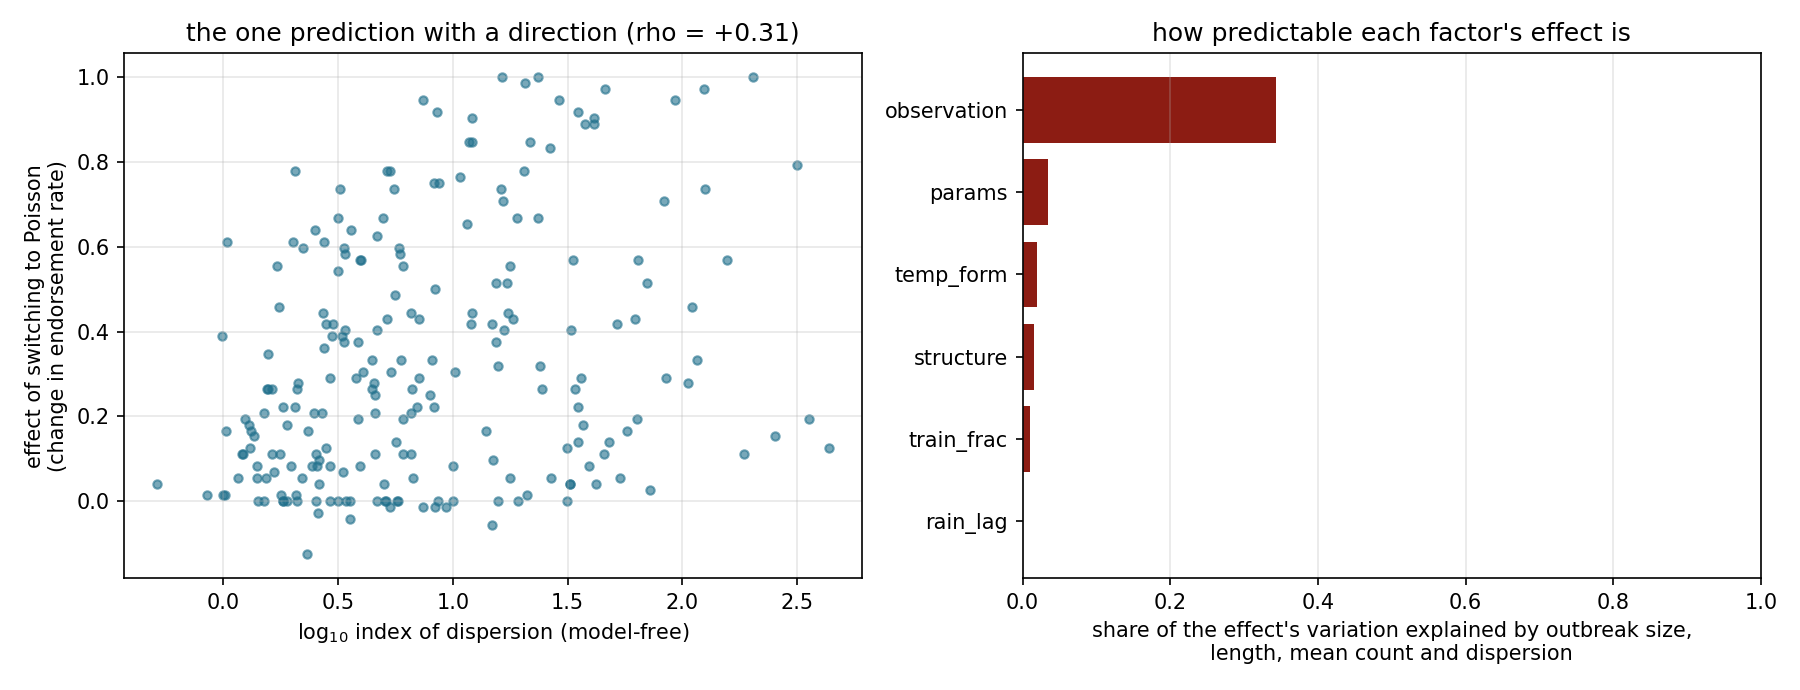
\includegraphics[width=\textwidth]{20_interaction_structure.png}
\caption{Left: the one prediction made in advance: the effect of assuming
Poisson counts against the model-free index of dispersion. Right: how much of
each factor's outbreak-to-outbreak variation four pre-fit descriptors account
for. Only the factor with a mechanism behind it is predictable, and only in part.}
\end{figure}

What survives, and is the stronger statement, is that the field's habit of
reaching first for a contextual explanation reaches for a term bounded at a
quarter, while three-fifths of the variation is not a property of the setting or
of the method but of what happens when a particular method meets a particular
epidemic. That term is invisible to both of the standard remedies. It is the
reason the recommendation this paper ends on is an interval computed within each
outbreak rather than a house style.

The specific contextual explanation on offer (that the association is
strongest where temperature varies most~\cite{kirk2024}) does not reproduce on
these data. Of eighteen correlations between six descriptions of each outbreak's
temperature regime and three outcomes, seven reach $p<0.05$ against about one
expected, but no $|\rho|$ exceeds 0.22 and \textbf{one} survives control of the
false-discovery rate: with the sign the wrong way round for the hypothesis.
Supplementary Section~S2 reports all eighteen.

\subsection{What this does to the number the field reports}
\label{sec:r0}

The verdict on climate forcing is a yes or a no, and a reader may reasonably feel
that a yes/no is a coarse thing to be unstable about. The same decomposition can
be applied to the quantity these papers actually report: the basic reproduction
number.

\begin{table}[htbp]
\centering
\caption{Variation in the estimated $R_0$ of the same 221 outbreaks. Reported
under four treatments of the long right tail, because the contrast and not the
exact figure is the finding.}
\begin{tabular}{lrrrr}
\toprule
& \multicolumn{2}{c}{Constant model} & \multicolumn{2}{c}{Climate model} \\
\cmidrule(lr){2-3}\cmidrule(lr){4-5}
Treatment & Between & Within & Between & Within \\
\midrule
Raw & 72.8\% & 27.2\% & 2.1\% & 97.9\% \\
Log scale & 71.6\% & 28.4\% & 19.8\% & \textbf{80.2\%} \\
Restricted to $R_0 \in [0.5, 20]$ & 72.8\% & 27.2\% & 17.1\% & 86.3\% \\
Restricted to $R_0 \le 10$ & 72.8\% & 27.2\% & 21.1\% & 81.4\% \\
\bottomrule
\end{tabular}
\end{table}

\textbf{The constant model's $R_0$ is mostly about the epidemic; the climate
model's is mostly about the analyst.} Under the constant model roughly 72\% of the
variation in estimated $R_0$ lies between outbreaks: the estimate is measuring
something that differs between epidemics, which is what it is for. Under the
climate model that falls to between 2\% and 21\% depending on how the long right
tail is handled, and the analytical share rises to 80--98\%. The contrast survives
every treatment we tried and is far larger than the differences between them.

Put on the scale a reader can weigh: the median outbreak's $R_0$ estimate ranges
over \textbf{1.31} across the 144 analyses, against a median estimate of
\textbf{1.29}. The spread induced by the choices is about the size of the quantity
being estimated.

The three-way partition of Section~\ref{sec:decomposition} says something the
two-way one cannot, and it is the practical question: could agreeing on a method
fix this?

\begin{table}[htbp]
\centering
\caption{Variation in estimated $R_0$, partitioned into what a convention could
reach (the analysis), and what it could not (the interaction). On the log scale,
which handles the long right tail; the raw scale is more extreme in the same
direction (0.5\% analysis, 97.4\% interaction under the climate model). The
climate-model row uses the 219 outbreaks whose $R_0$ is positive and finite under
every analysis, which is why its ``outbreak'' share reads 22.5\% here against
19.8\% in the table above, computed on all 221.}
\begin{tabular}{lrrr}
\toprule
& Outbreak & Analysis & Interaction \\
\midrule
$R_0$, constant model & 71.6\% & 5.3\% & 23.0\% \\
$R_0$, climate model & 22.5\% & \textbf{8.4\%} & \textbf{69.1\%} \\
\bottomrule
\end{tabular}
\end{table}

\textbf{No convention would fix it.} The analysis main effect for $R_0$ is about a
twentieth under either model, there is no systematically high-reading method to
stop using. What adding climate terms does is move variation out of the outbreak
and into the \emph{interaction}, which rises from 23\% to 69\%. The instability in
the number this field reports is not a house style anyone could adopt their way
out of; it is specific to the meeting of a method with an epidemic, and the only
report that carries it is one made within the outbreak.

This connects to the identifiability result in the appendix from the other
direction. There, adding climate parameters to a short series destroyed the
identifiability of the population at risk, which the simpler model recovered to
within a factor of two. Here the same addition destroys the stability of $R_0$.
The climate terms are not free: they are paid for in the precision of everything
else in the model, and that cost is not usually reported because it is not usually
looked for.

\subsection{How often the verdict changes, measured two ways}

\begin{table}[htbp]
\centering
\caption{Stability of the in-sample verdict within each outbreak.}
\begin{tabular}{lrr}
\toprule
& Windows & Share \\
\midrule
Always favours climate forcing & 18 & 8.1\% \\
Never favours climate forcing & 0 & 0.0\% \\
\textbf{Verdict changes with the choices} & \textbf{203} & \textbf{91.9\%} \\
\bottomrule
\end{tabular}
\end{table}

Bootstrapping over windows, the independent units, gives a 95\% interval of
87.8--95.5\%. Among unstable windows the median split is 107 of 144 combinations
in favour. The instability appears in every well-represented country, ranging
from 85\% to 100\%.

\paragraph{That figure is not comparable across studies, and we do not rely on
it.} Asking whether \emph{any} two combinations disagree becomes easier the more
combinations there are: a design with 144 cells will exceed one with 24 even if
nothing about the evidence has changed. Since this study grew its own design
twice, the point applies to it directly.

We therefore report alongside it the probability that two analyses of the same
outbreak, drawn at random, reach opposite verdicts. With $p$ the proportion of
analyses favouring climate forcing, that is $2p(1-p)$: a function of the
proportion and not of how finely the space was enumerated, zero for a unanimous
outbreak and one half for an evenly split one. Across the 221 outbreaks it is
\textbf{29.8\%} (median 34.6\%), and it exceeds 25\% in 61.1\% of them.

\begin{table}[htbp]
\centering
\caption{Every design this study ran. The share of outbreaks where some pair
disagrees climbs with the number of cells; the pairwise probability does not.}
\begin{tabular}{lrrrr}
\toprule
Design & Combinations & Outbreaks & Some pair disagrees & P(two disagree) \\
\midrule
Four factors & 24 & 236 & 82.6\% & 29.9\% \\
Five factors & 48 & 234 & 88.0\% & 31.4\% \\
\textbf{Six factors} & \textbf{144} & \textbf{221} & \textbf{91.9\%} & \textbf{29.8\%} \\
\bottomrule
\end{tabular}
\end{table}

Each factor was added to close a gap the previous version had named in its own
limitations section, not sought once a result was known; the fixed
epidemiological parameters, added for that reason, turn out to be the weakest
factor of the six. The invariant statistic is flat across all three designs at
about 30\%, which is the figure we ask readers to carry away.

\subsection{Statistical conventions dominate; the biology does not}

\begin{table}[htbp]
\centering
\caption{Effect of each choice, paired within window so that differences in
series length or case count cannot drive the comparison.}
\begin{tabular}{lrr}
\toprule
Choice varied & Verdicts flipped & P(climate wins) before $\to$ after \\
\midrule
\multicolumn{3}{l}{\emph{Statistical conventions}} \\
\textbf{Negative binomial $\to$ Poisson} & \textbf{34.3\%} & $0.570 \to 0.900$ \\
75\% $\to$ 100\% of the series & 20.7\% & $0.702 \to 0.769$ \\
\midrule
\multicolumn{3}{l}{\emph{Covariate handling}} \\
Rainfall lag 3 $\to$ 7 weeks & 15.8\% & $0.734 \to 0.738$ \\
Brière $\to$ log-linear temperature & 11.5\% & $0.696 \to 0.774$ \\
Rainfall lag 3 $\to$ 5 weeks & 11.0\% & $0.734 \to 0.733$ \\
\midrule
\multicolumn{3}{l}{\emph{Epidemiological content}} \\
Host--vector $\to$ human-only SEIR & 9.9\% & $0.738 \to 0.727$ \\
Host--vector $\to$ thermal mortality & 9.4\% & $0.738 \to 0.741$ \\
\textbf{Central $\to$ alternative fixed parameters} & \textbf{3.1\%} & $0.735 \to 0.736$ \\
\bottomrule
\end{tabular}
\end{table}

The factors fall into three groups, and the ordering is the result. The
\emph{statistical conventions} (which likelihood, how much of the series to
fit) flip 21\% and 34\% of verdicts. The \emph{covariate handling} follows at
11--16\%. The \emph{epidemiological content} (which transmission mechanism, and
what the biological parameters are) comes last at 3--10\%. On this evidence the
question is answered by the statistics rather than by the biology.

The two factors added specifically to answer the objection that the study was
testing a toy model are among the weakest. Replacing the host--vector formulation
with a directly transmitted SEIR flips 9.9\%; replacing it with a host--vector
model whose mosquito mortality follows temperature flips 9.4\%. Moving the fixed
epidemiological parameters (lifespan, incubation periods, vector-to-host ratio) to the other end of their published ranges flips \textbf{3.1\%} and moves the
endorsement probability by 0.001. We expected that factor to matter and it does
not.

\label{sec:mechanism}
Assuming Poisson counts raises the probability of endorsing climate forcing from
0.57 to 0.90. Two mechanisms could produce that, and they make opposite
predictions, so we measured rather than argued.

The first is the one usually given, and the one an earlier draft of this paper
gave: Poisson treats ordinary noise as a large residual, the fit chases individual
weeks, and the climate covariates supply the flexibility to do it. If so their
coefficients should be pushed harder under Poisson. \textbf{They are not.} Paired
within outbreak and within every other choice, the median $|a_{\mathrm{temp}}|$ is
0.092 under a negative binomial and 0.097 under Poisson, and is larger under
Poisson in 40\% of 15{,}912 pairs: less often than chance. For
$|a_{\mathrm{rain}}|$ it is 46\%. The climate model does the same thing under both
likelihoods.

What changes is what the criterion pays for it. The climate model nests the
constant one, so it fits at least slightly better always; the question is only
whether the improvement clears two parameters' worth of penalty. Without a
dispersion parameter to absorb the residual, the same improvement buys far more
log-likelihood: the median $\Delta$AIC is $-1.6$ under a negative binomial and
$\mathbf{-68.9}$ under Poisson, a ratio of \textbf{13} where the two agree in
sign, and larger in magnitude under Poisson in 90\% of pairs. The asymmetry is
near-total: climate forcing wins under both in 56.4\% of pairs, under Poisson
alone in \textbf{33.6\%}, and under the negative binomial alone in \textbf{0.6\%}.

So the mechanism is not that Poisson makes the model chase noise. It is that
Poisson makes the criterion generous, and it is generous in one direction only.
The dispersion it ignores is real, and is expected: infectious disease counts
are overdispersed by individual variation in transmission~\cite{lloydsmith}, and
the standard remedies for it in count regression are long
established~\cite{mccullagh}. Taking residuals about a five-week moving
average (a measure independent of any transmission model) these series have
a median index of dispersion of \textbf{5.7}, quartiles 2.6 and 19.1, and a
quarter above 20. A week of 2{,}000 cases that Poisson treats as accurate to
$\pm 45$ is accurate to about $\pm 107$.

A reader may object that Poisson is not a defensible choice at all on
overdispersed counts, and that including it inflates the instability by admitting
a cell that should never have been in the multiverse. Two things answer this. The
field uses it, in the proportion given in Section~3: a large minority rather
than a majority, which is the honest reading and still enough that a multiverse
excluding it would not describe the literature it is about. Where the two are
compared head to head on mosquito-borne outbreak data the negative binomial is
the better model~\cite{nbcompare}. And the result does not depend on
it. Restricting the entire study to negative-binomial fits (discarding half the
factorial as indefensible) still leaves \textbf{79.6\%} of outbreaks changing
verdict (95\% CI 75--85), because the remaining five choices continue to move it.
The observation model is the largest lever, not the only one.

The rainfall lag behaves differently and is worth separating. It flips one verdict
in six while moving the average by 0.004. That is variance injected into a
conclusion by an arbitrary choice, without any systematic effect to justify it.

\begin{figure}[htbp]
\centering
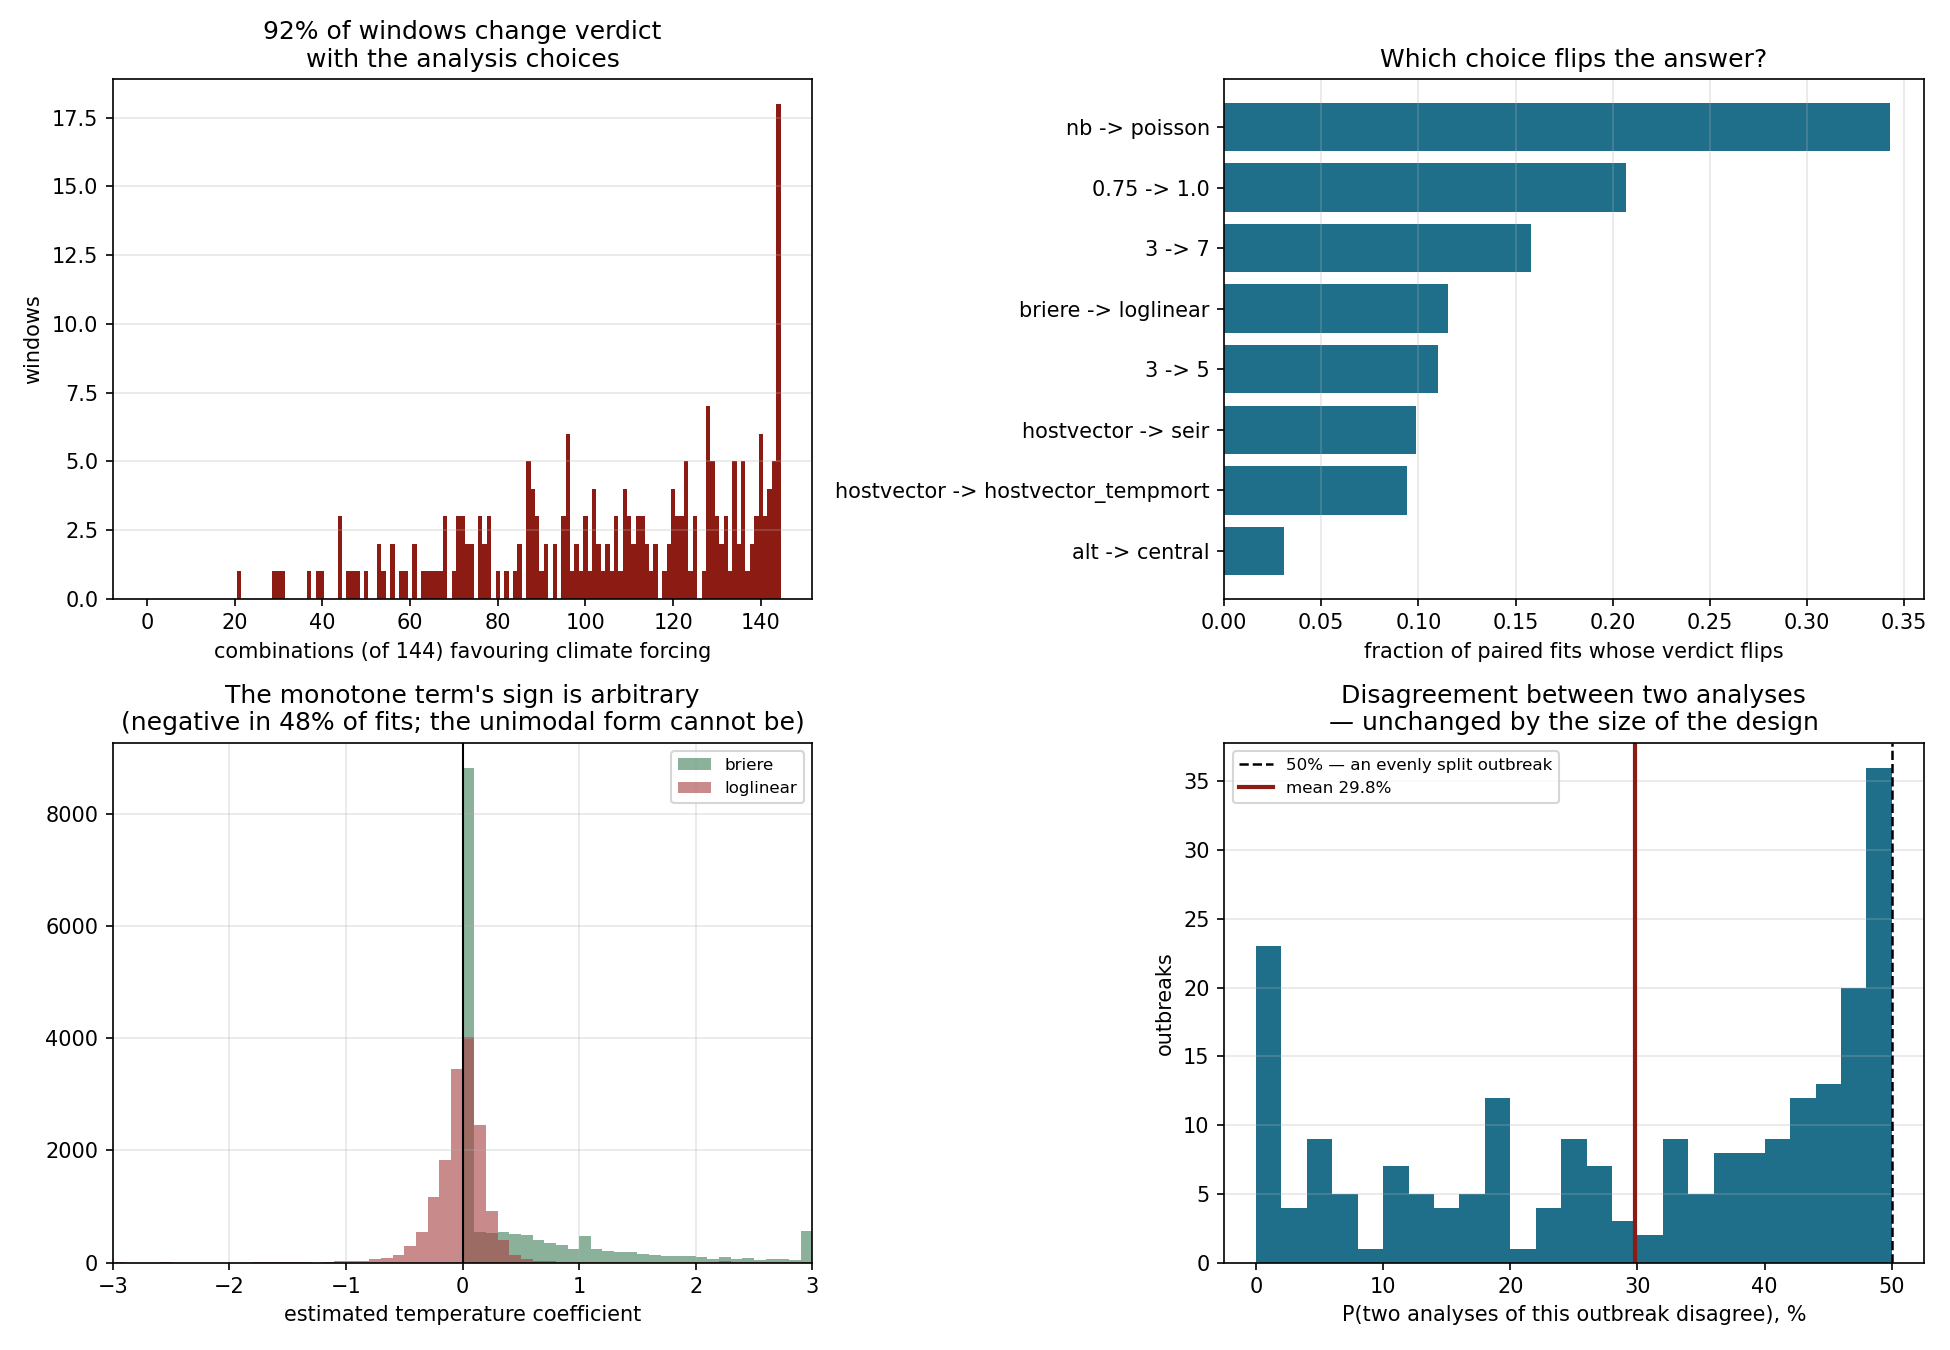
\includegraphics[width=\textwidth]{12_global_robustness.png}
\caption{The four results of the factorial. Top left: how many of the 144
analyses favour climate forcing, per outbreak: the mass sits well short of
unanimity at either end. Top right: the share of paired comparisons each choice
flips, which separates the statistical conventions from the epidemiological
content. Bottom left: the estimated temperature coefficient by parameterisation,
clipped to $\pm 3$; the monotone form is negative in half of all fits and the
unimodal form cannot be. Bottom right: the probability that two analyses of one
outbreak disagree, the statistic that does not grow with the design.}
\label{fig:main}
\end{figure}

\subsection{The specification curve}
\label{sec:speccurve}

Figure~\ref{fig:speccurve} shows the multiverse directly, in the two forms the
question takes.

\textbf{Within one outbreak.} The left panel draws the most evenly split window in
the study (Jamaica, July 2023) where exactly 72 of the 144 specifications
favour climate forcing and 72 favour the constant model. The $\Delta$AIC values
run from $-337$ to $+4$. One analyst, following defensible
conventions, would report overwhelming evidence for climate-driven transmission
in this epidemic; another, following different but equally defensible
conventions, would report no evidence at all. The dot matrix below shows why: the
observation-model row splits the panel exactly, every Poisson specification lying
on the climate side and every negative binomial on the other.

\textbf{Across outbreaks.} The right panel gives each specification the whole
study and asks how often it endorses climate forcing. If the choices were
interchangeable the result would be a flat line. The most credulous specification
 (Poisson counts, a log-linear temperature term, a three-week rainfall lag, the
first 75\% of the series, an SEIR structure and the central parameter set)
endorses climate forcing in \textbf{95.9\%} of outbreaks. The least credulous
differs from it in exactly two of the six, the observation model and the
temperature form: negative binomial and Brière, with the same lag, the same
fraction, the same structure and the same parameters. It endorses climate forcing
in \textbf{39.8\%}.
That is a spread of \textbf{56 percentage points} between two analyses of the same
data, neither of which any reviewer would reject on its face.

This is the finding stated as a rate rather than as a count of flips, and it is
the form in which it bears on reading the published literature: a paper reporting
that climate forcing improved the fit has told the reader where in this range its
analysis sat only if it stated all six choices, which such papers generally do
not.

\begin{figure}[htbp]
\centering
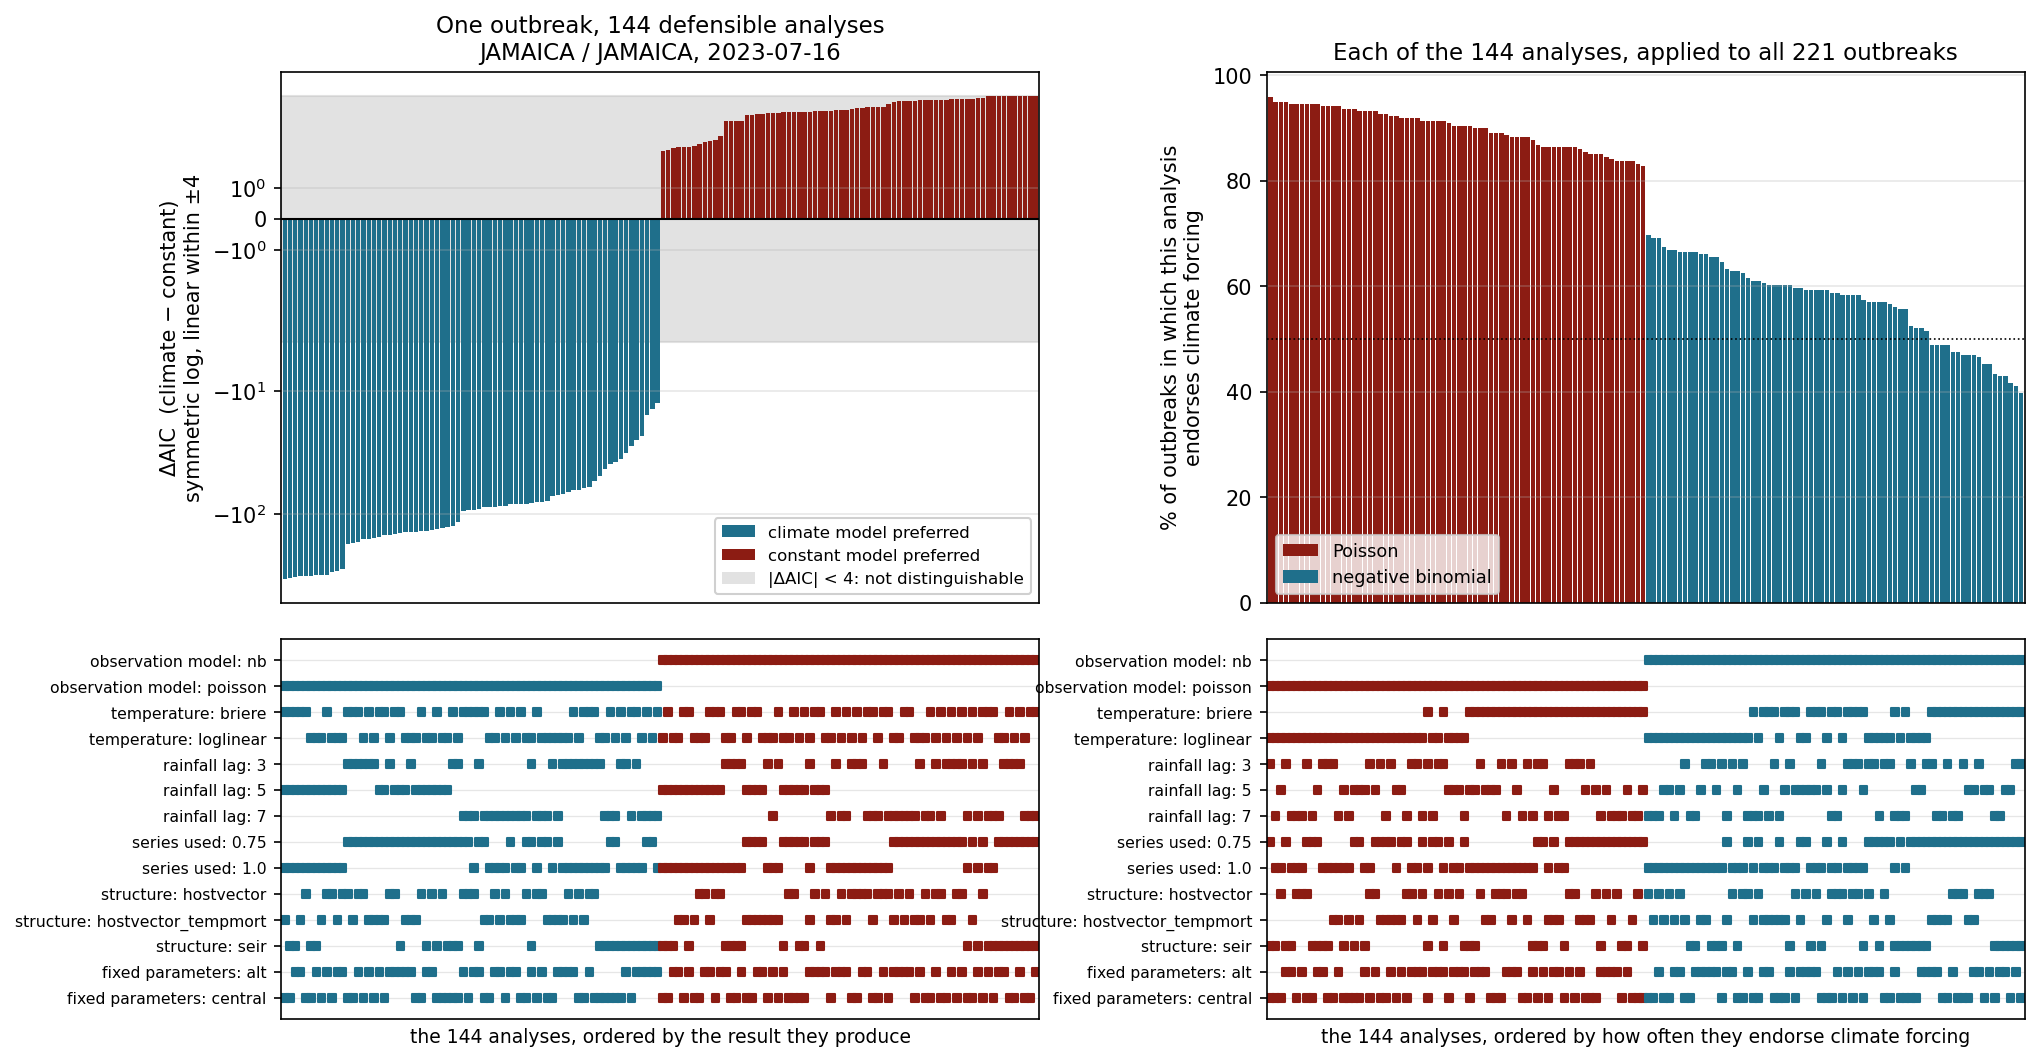
\includegraphics[width=\textwidth]{17_specification_curve.png}
\caption{The specification curve. Left: all 144 analyses of a single outbreak,
ordered by the result they produce, on a symmetric-log scale that is linear
within $\pm 4$ so that both directions remain visible. Right: each of the 144
analyses applied to all 221 outbreaks, ordered by how often it endorses climate
forcing. Lower panels mark which choices each analysis used.}
\label{fig:speccurve}
\end{figure}

\subsection{Out-of-sample validation halves endorsement but not instability}

On three Pakistani windows examined first, held-out deviance preferred the
constant model in every configuration, suggesting that validation was the stable
criterion. Across 221 outbreaks that does not hold.

\begin{table}[htbp]
\centering
\caption{In-sample and out-of-sample compared on the same fits.}
\begin{tabular}{lrr}
\toprule
& Unstable within window & Climate preferred \\
\midrule
In-sample (AIC) & 84.7\% & 70.3\% of fits \\
Out-of-sample (held-out deviance) & 90.6\% & 36.3\% of fits \\
\bottomrule
\end{tabular}
\end{table}

Validation halves the rate at which climate forcing is endorsed (a large and
useful reduction in false positives), but leaves the verdict at least as
dependent on the remaining choices: 90.6\% of outbreaks are unstable
out-of-sample against 84.7\% in-sample. It is a corrective, not a solution.
Earlier versions of this study, on smaller designs, found the two rates equal;
enlarging the design moves the out-of-sample figure above the in-sample one,
which is the opposite of what a remedy would do.

\subsection{The conventional temperature term reports an arbitrary sign}

\begin{table}[htbp]
\centering
\caption{Estimated temperature coefficient by parameterisation, 15{,}912 fits each.}
\begin{tabular}{lrrr}
\toprule
Parameterisation & Mean & Median & Negative in \\
\midrule
Brière (unimodal, from vector thermal biology) & $+0.583$ & $+0.021$ & \textbf{0.0\%} \\
Log-linear (conventional) & $-0.000$ & $+0.000$ & \textbf{48.5\%} \\
\bottomrule
\end{tabular}
\end{table}

The log-linear coefficient is negative in essentially half of all fits and
positive in the rest, averaging to nothing. The explanation usually offered is
that a monotone term fitted to a season whose temperature falls while cases rise
must return a negative coefficient whatever the biology, so the sign is a property
of the calendar. We tested it rather than repeating it. Against the temperature
trend over each outbreak's growth phase the estimate correlates at
$\rho = +0.25$ ($p = 1\times10^{-4}$): where temperature falls during growth the
coefficient is negative in 52\% of outbreaks, where it rises, in 32\%.

So the direction is as claimed and the size is not. The calendar tilts the sign
without setting it, which leaves most of the sign unexplained, and a
coefficient whose sign is half calendar and half unaccounted for is not a
measurement of anything. A unimodal response cannot produce a negative value at
all, because it has no direction to choose.

\subsection{A remedy, and it is nearly free}
\label{sec:remedy}

\begin{table}[htbp]
\centering
\caption{Candidate decision rules. Both columns matter: a rule that is never
wrong because it never speaks is not a remedy.}
\begin{tabular}{lrrrr}
\toprule
Rule & Some pair disagrees & 95\% CI & P(two disagree) & Answers for \\
\midrule
Sign of $\Delta$AIC (conventional) & 91.9\% & 88--96\% & 29.8\% & 100\% \\
$|\Delta\mathrm{AIC}| > 2$ & 89.6\% & 86--93\% & 24.9\% & 100\% \\
$\boldsymbol{|\Delta\mathrm{AIC}| > 4}$ & 39.8\% & 33--45\% & \textbf{4.0\%} & \textbf{100\%} \\
$|\Delta\mathrm{AIC}| > 10$ & 37.0\% & 32--44\% & 4.5\% & 97.7\% \\
$|\Delta\mathrm{AIC}| > 20$ & 34.9\% & 29--41\% & 4.7\% & 95.9\% \\
Negative binomial only & 79.6\% & 75--85\% & n/a & 100.0\% \\
Negative binomial, $|\Delta\mathrm{AIC}| > 10$ & 20.0\% & 14--25\% & n/a & 74.7\% \\
All 144 combinations must agree & 0.0\% & n/a & n/a & 8.1\% \\
\bottomrule
\end{tabular}
\end{table}

Read the two instability columns together, because separately each misleads.
Between margins of 2 and 4 the \emph{pairwise} disagreement collapses from 24.9\%
to \textbf{4.0\%} while the rule still answers for every outbreak: on that scale
the remedy works exactly as it did on the smaller designs, and at the same place.
The share of outbreaks in which \emph{some} pair still disagrees falls only from
90\% to 40\%, but that column is the one that grows with the size of the design,
and it is not comparable with the 6.9\% obtained from 48 combinations.

Both are true and the pair is the finding. Where dissent survives a margin of 4,
the dissenting minority is small: a median of 3 of the 100 analyses still
speaking, 2.8\% of them. A margin makes the surviving disagreement rare within an
outbreak without making it absent from the study.

The interpretation is direct: \textbf{almost all of the instability lies in
comparisons where $|\Delta\mathrm{AIC}| < 4$}, that is, where the models were
never distinguishable. Burnham and Anderson's long-standing guidance treats
$\Delta$AIC below 4 as substantial support for both models~\cite{burnham}. The
recommendation is therefore not new; what is new is the measured cost of not
following it.

Two alternatives fare worse. Requiring unanimity across the factorial is perfectly
stable and speaks for one outbreak in twelve. Fixing the observation model alone
 (the single largest lever) still leaves 80\% of outbreaks with some
disagreement, because the remaining choices continue to move the verdict.
Combining the two does better: restricting to the negative binomial and requiring
$|\Delta\mathrm{AIC}| > 10$ leaves 20\%, and speaks for three outbreaks in
four.

\begin{figure}[htbp]
\centering
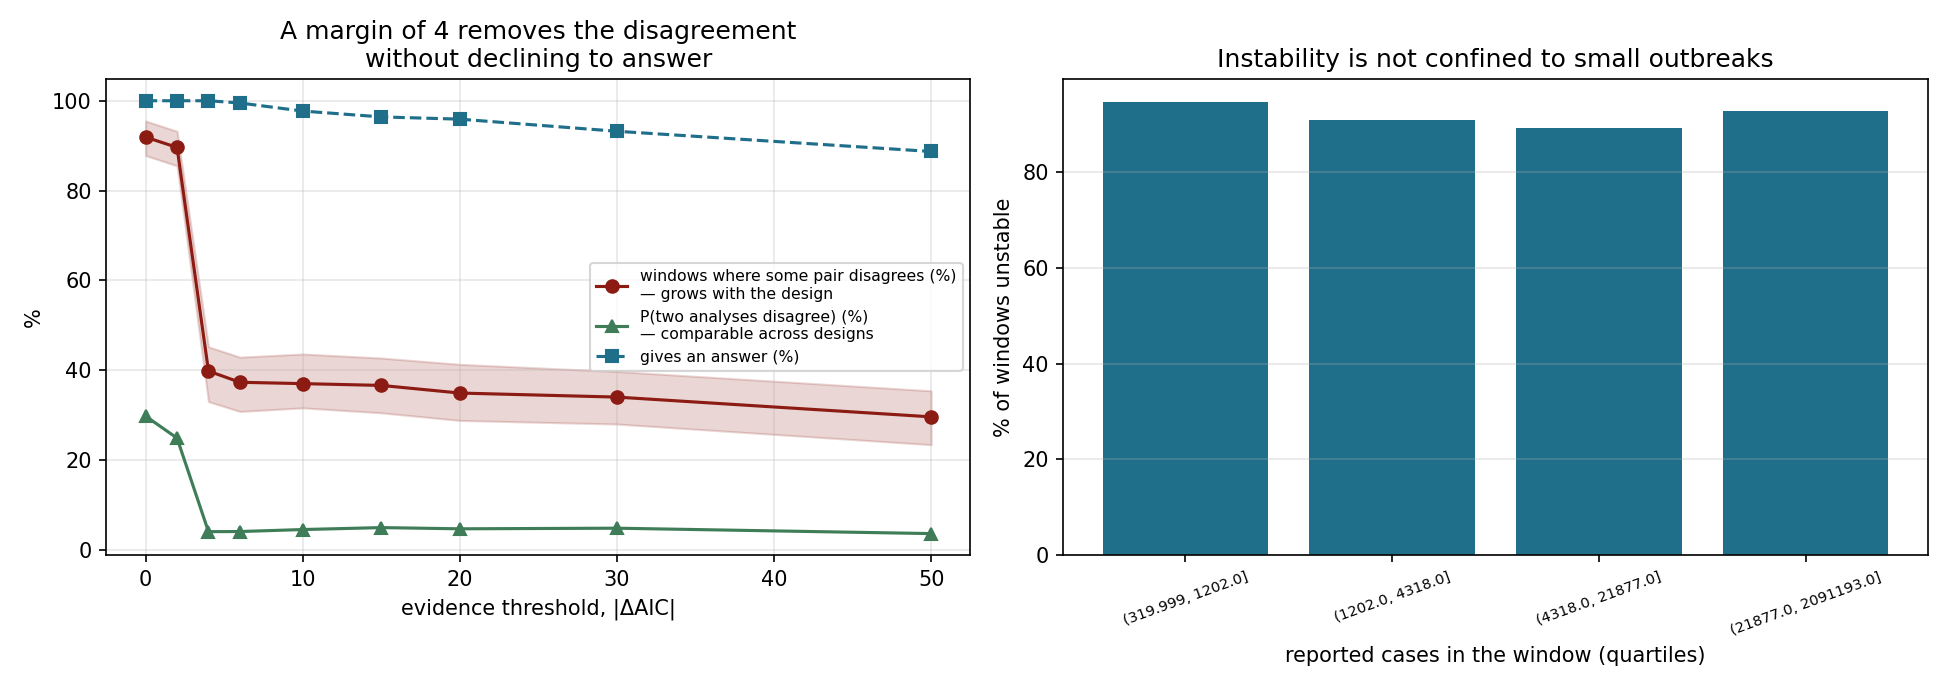
\includegraphics[width=\textwidth]{13_stability_remedy.png}
\caption{Left: the effect of an evidence margin on both scales, with the share of
outbreaks still receiving a verdict. The share where some pair disagrees (dark), and the probability that two analyses disagree (green) both collapse between 2 and
4, but to very different levels, and only the second is comparable with the
smaller designs. Right: instability by quartile of reported cases.}
\end{figure}

AIC, BIC and the likelihood-ratio test are thresholds on the same quantity at
different points, and strictness makes matters worse monotonically: instability
is 91.9\% under AIC's sign, 95.0\% under a likelihood-ratio test at $p<0.05$ and
96.8\% under BIC. A $\pm 4$ band on the BIC scale still leaves 90.5\% unstable,
because BIC's extra penalty shifts the abstention band off centre. Supplementary
Section~S3 gives the comparison; what matters is not how strict a rule is but
whether it abstains symmetrically about zero.
Two facts hold at once: the choices move $\Delta$AIC by a median of
\textbf{804} units within a single outbreak, roughly fifty-six times the median
difference being read as evidence, yet in \textbf{60.2\%} of outbreaks every
dissenting combination dissents on evidence weaker than $\Delta$AIC $=4$. Most of
that enormous movement stays on one side of zero. Supplementary Section~S4 gives
the full account, including why a stricter threshold cannot reach the confident
dissent that survives.
\subsection{How often is the verdict wrong, and in which direction?}
\label{sec:errors}

Everything above measures disagreement, which shows that something is wrong
without showing which answer is wrong: on real data there is no truth to compare
against. We therefore simulated counts from models whose answer is known, using
each window's own fitted parameters, its own climate series and its own estimated
dispersion, and ran the full factorial on them. Eighty windows, two truths, all
144 combinations: 23{,}000 fits.

The two truths are matched on mean transmission. Switching the climate
coefficients on multiplies $\beta(t)$ by a factor whose average is not one, so an
unadjusted alternative would differ from the null in overall transmission
intensity as well as in whether transmission varies, and in an earlier version
of this analysis the raised $R_0$ made the generating integration diverge for 21
of 59 windows, so power was estimated only where a strong effect happened not to
break the model. Rescaling $\beta_0$ by the mean of the climate multiplier
isolates the contrast the study is about and leaves both arms covering the same
windows.

\begin{table}[htbp]
\centering
\caption{False positives (data generated with no climate effect), and power (data
generated with an effect of realistic size). Separation is power minus
false-positive rate: how far the rule distinguishes the two truths, as opposed to
how often it says yes.}
\begin{tabular}{llrrr}
\toprule
Observation model & Rule & False positives & Power & Separation \\
\midrule
Poisson & sign of $\Delta$AIC & 85.7\% & 95.3\% & \textbf{10 pts} \\
Poisson & margin 4 & 78.6\% & 93.5\% & 15 pts \\
Poisson & margin 24 (its best) & 58.8\% & 86.6\% & 28 pts \\
\midrule
\textbf{Negative binomial} & \textbf{sign of $\Delta$AIC} & 18.7\% & 73.4\% & \textbf{55 pts} \\
Negative binomial & margin 4 & 6.2\% & 61.8\% & 56 pts \\
Negative binomial & margin 12 & 3.3\% & 43.3\% & 40 pts \\
\bottomrule
\end{tabular}
\end{table}

\textbf{A Poisson observation model does not discriminate.} On data containing no
climate signal it endorses climate forcing six times in seven. Its 95\% power is
not a virtue next to an 86\% false-positive rate: the procedure is agreeing with
almost everything. Over every margin tested its best separation is 28 points, and
reaching even that requires abstaining below $|\Delta\mathrm{AIC}| = 24$.

\textbf{The observation model is worth 45 points of separation.} Switching to a
negative binomial moves separation from 10 to 55 at the identical decision rule.
Nothing else examined here approaches that.

\textbf{The margin is a specificity dial, not an improvement.} On the negative
binomial it trades power against false positives along the same curve rather than
shifting the curve outward, separation is 54.7 at margin 0 and 55.6 at margin
4, essentially unchanged while false positives fall from 18.7\% to 6.2\%. It is
the right control when a false positive costs more than a miss, and it is not a
substitute for the observation model: applied to Poisson counts a margin of 4
still leaves 79\% false positives.

This bears on the empirical result, but less than an earlier draft claimed.
Poisson endorsed climate forcing in 90.0\% of real fits and the negative binomial
in 57.0\%. Pairing the two within outbreak and within every other choice, Poisson
endorses where the negative binomial does not in \textbf{33.6\%} of real pairs;
that same discordant cell occurs in \textbf{67.1\%} of simulated pairs when no
climate effect exists and \textbf{23.3\%} when one does. The cell is diagnostic
 (three times as common under the null), but the real rate sits nearer the arm
that contains an effect than the arm that does not. The earlier draft stated that
85.7\% of Poisson endorsements would occur on data with no effect, and that most
of the gap between the observation models was therefore not detection. Neither
follows: 85.7\% is the false-positive rate under a null truth and not a share of
endorsements, and a mixture read off these three rates puts the null fraction
nearer a quarter than a majority. We report the rates and decline the inference,
for the same reason given below: the simulated effect size comes from these
same fits.

\paragraph{The instability is not manufactured by running 144 analyses.} The
arithmetical objection to the headline is that with enough analyses something will
always disagree. The simulation answers it, because here the truth is known and
the factorial is identical in both arms. Measured on the scale that does not grow
with the design, two analyses of the same simulated outbreak reach opposite
verdicts \textbf{44.5\%} of the time when no climate effect is present (close to
the 50\% ceiling, which is what pure coin-flipping looks like), and
\textbf{18.6\%} when a real effect of realistic size is. The truth more than
halves the disagreement, so the design is not generating it out of nothing.

The more uncomfortable half is the 18.6\%. Even when a genuine climate effect is
present, at a size drawn from these epidemics' own fitted parameters, two
defensible analyses still reach opposite conclusions almost one time in five. The
instability is not only a symptom of weak evidence; a real signal of ordinary size
does not survive it either.

\paragraph{The remedy holds under both truths.} Applying the recommended rule to
the same simulated data (abstain within $|\Delta\mathrm{AIC}| = 4$) reduces
pairwise disagreement from 44.5\% to \textbf{1.8\%} where no climate effect
exists, and from 18.6\% to \textbf{4.3\%} where one does. It works in both cases
and works slightly less completely where an effect exists, which is the expected
direction: a real effect produces large $|\Delta\mathrm{AIC}|$, so some dissent
falls outside the abstention band. A margin removes disagreement about comparisons
too close to call; it cannot remove disagreement about a difference the analyses
genuinely disagree about.

\paragraph{Which arm do the real outbreaks resemble? A one-number answer cannot
say.} It is tempting to compare the real data with the two simulated arms, and two
attempts to do so failed. On pairwise disagreement the real outbreaks sit between
(29.8\%, against 44.5\% with no effect and 18.6\% with one); under the margin-4
rule the ordering reverses (4.0\%, against 1.8\% and 4.3\%). An earlier version of
this study, using the design-dependent share of unstable windows, reported that the
real data resembled the no-effect arm; that reading did not survive the invariant
measure and was withdrawn.

The reason both attempts failed is now visible: the arms differ in three
components and each of those statistics compresses them to one. Partitioning the
same three datasets the same way separates them.

\begin{table}[htbp]
\centering
\caption{The three-way partition applied to both simulated arms and to the real
outbreaks. Same windows, same 144 analyses, same fitted parameters; only the truth
differs between the first two rows.}
\begin{tabular}{lrrr}
\toprule
& Outbreak & Analysis & Interaction \\
\midrule
Simulated, no climate effect & 10.9\% & \textbf{47.0\%} & 42.1\% \\
Simulated, real effect present & 28.6\% & 10.3\% & 61.1\% \\
\midrule
\textbf{Real outbreaks} & \textbf{23.5\%} & \textbf{15.9\%} & \textbf{60.6\%} \\
\bottomrule
\end{tabular}
\end{table}

\textbf{The analysis main effect is what discriminates, and it does so sharply.}
Where there is nothing to detect it is the largest of the three at 47\%, which is
what should happen: with no signal the answer is whatever the convention gives, and
the convention does not vary by window. Where a real effect is present it collapses
to 10\%. The real outbreaks read \textbf{15.9\%} (with the effect arm, four
times away from the null arm), and their outbreak and interaction shares land
within five points of that arm on both.

We report this as evidence and not as proof. The simulated effect size is drawn
from these same fits, the two arms are not a calibrated mixture of what the world
contains, and a fingerprint matching one arm does not establish that every outbreak
in it carries a signal. What it does establish is that the real data does not carry
the signature of a literature detecting nothing, which is the reading the earlier
withdrawn sentence had pointed toward. It is also consistent with
Section~\ref{sec:ownanswer}, where our own rule gives a clear verdict for 137
outbreaks and 86\% of those support climate forcing.

\begin{figure}[htbp]
\centering
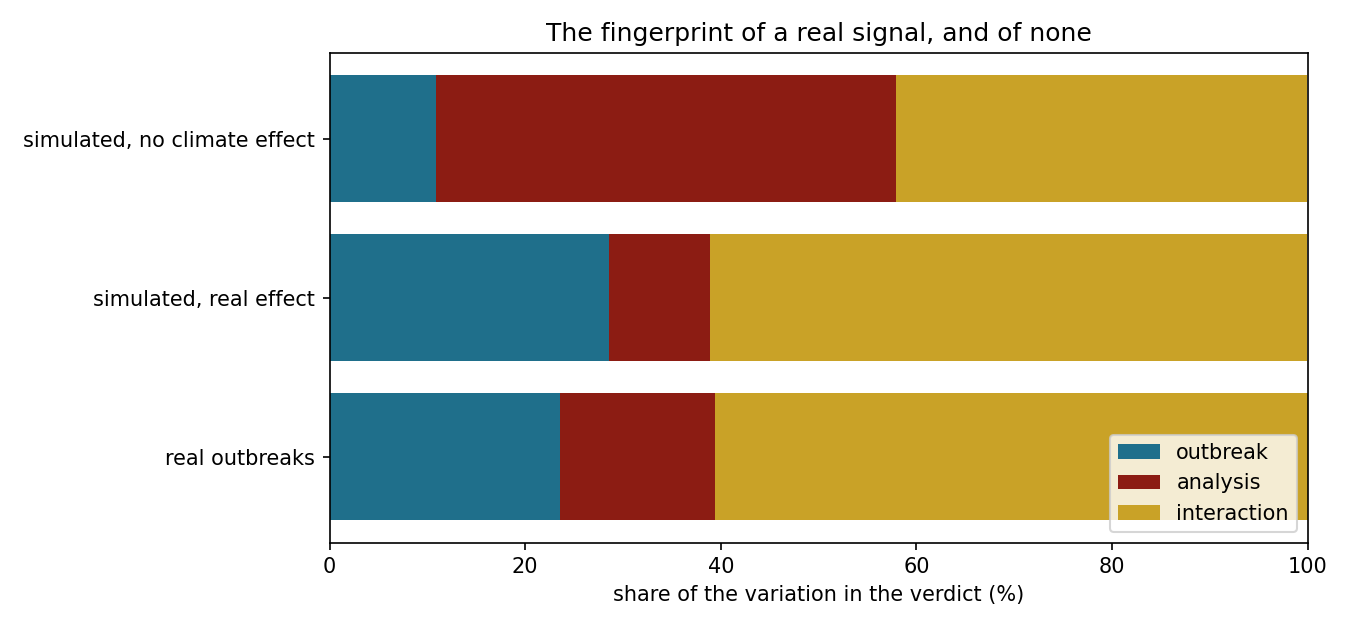
\includegraphics[width=0.85\textwidth]{21_decomposition_under_truth.png}
\caption{The fingerprint of a real signal and of none. The analysis main effect
(centre band) is the discriminating component: largest where there is nothing to
detect, small where there is something.}
\end{figure}

\begin{figure}[htbp]
\centering
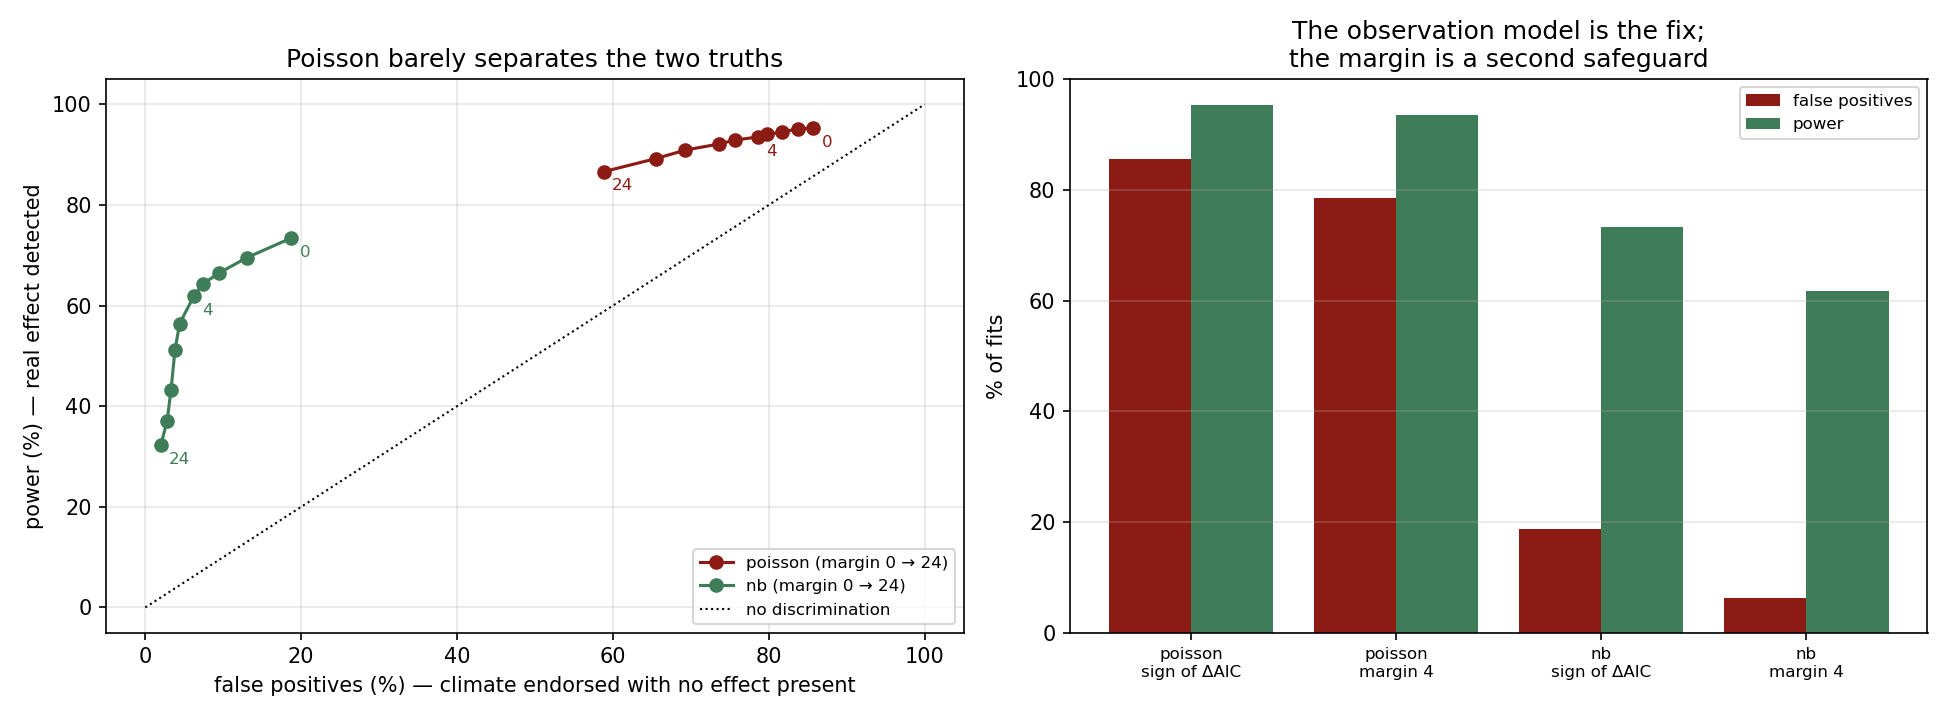
\includegraphics[width=\textwidth]{16_operating_characteristics.png}
\caption{Left: power against false positives as the decision margin varies from
0 to 24. The Poisson curve lies close to the diagonal of no discrimination.
Right: the same four rules as rates.}
\end{figure}

\subsection{The intervals do not cover, and an interval that does}
\label{sec:coverage}

Everything above concerns which model is chosen. A paper also reports a number
with an interval around it, and that interval makes a specific promise: that it
contains the true value 95 times in 100. The promise is testable here, because
the truth is set by us.

Counts were simulated from each window's own fitted parameters with the Brière
temperature exponent set to $1.0$ and the rainfall coefficient to $0.30$, and
every Brière combination was asked to recover them, 80 outbreaks, 72
combinations each, 5{,}760 fits. A conventional analysis reports one estimate and
$\hat\theta \pm 1.96\,\mathrm{SE}$ from one set of choices. Coverage is computed
over every cell, so the figure describes what an analyst drawing any defensible
set of choices would obtain, not one arbitrary choice.

\begin{table}[htbp]
\centering
\caption{Coverage of a nominal 95\% interval. The multiverse interval combines
all analyses of an outbreak by Rubin's rules, whose within- and between-analysis
variance decomposition applies unchanged here: several analyses of one dataset,
each with its own estimate and its own sampling variance.}
\begin{tabular}{lrrr}
\toprule
Interval & Temperature exponent & Rainfall coefficient & Transmission coefficient \\
\midrule
Conventional, one analysis & 82.9\% & \textbf{71.2\%} & \textbf{78.0\%} \\
\textbf{Multiverse (Rubin)} & \textbf{100.0\%} & \textbf{97.5\%} & \textbf{100.0\%} \\
\bottomrule
\end{tabular}
\end{table}

\textbf{A conventional 95\% interval for the rainfall coefficient contains the
truth 71\% of the time.} For the temperature exponent it manages 83\%, and for the
transmission coefficient (which fixes $R_0$ within a structure, so the two have
the same coverage) \textbf{78\%}. All three are below the promise, and the
shortfall is not a subtlety of the asymptotics: a conventional interval reports the
square root of the within-analysis variance and behaves as though the
between-analysis variance were zero, when for the rainfall coefficient the two are
of the same size.

The point estimates are no better behaved. The ratio of the estimated transmission
coefficient to the truth has a median of $1.27$ and an interquartile range of
$0.74$ to $2.59$: in the middle half of analyses the reported $R_0$ is between
three-quarters and two and a half times the value that generated the data. That is
the number this field reports, on data whose answer we set ourselves.

\textbf{Combining the analyses restores the promise.} Rubin's
rules~\cite{rubin} give
$\bar\theta \pm t\sqrt{W + (1 + 1/m)B}$, with $W$ the mean within-analysis
variance and $B$ the variance between the estimates. Coverage becomes 97.5\% and
100.0\%, at the cost of an interval 1.5 to 2.2 times wider. The 100\% is
conservative rather than exact and we report it as such; with $m = 72$ analyses
and a long-tailed estimate distribution, $B$ is generous.

That trade is the whole recommendation in one line. The narrow interval is not
more informative than the wide one; it is the same information with a promise
attached that it does not keep.

\paragraph{Eight analyses are enough.} A recommendation costing 288 fits per
outbreak would be admired and not used, so we asked how far it can be cheapened.
Drawing $m$ analyses at random from an outbreak's 72 and combining only those:

\begin{table}[htbp]
\centering
\caption{Coverage of the multiverse interval against the number of analyses
combined, averaged over 20 random draws per outbreak.}
\begin{tabular}{lrrrrrr}
\toprule
Analyses combined & 2 & 4 & \textbf{8} & 16 & 24 & 72 \\
\midrule
Rainfall coefficient & 91.0\% & 96.2\% & \textbf{97.3\%} & 97.6\% & 97.6\% & 97.5\% \\
Temperature exponent & 94.9\% & 98.6\% & \textbf{100.0\%} & 100.0\% & 100.0\% & 100.0\% \\
Transmission coefficient & 91.7\% & 97.1\% & \textbf{98.9\%} & 99.9\% & 99.9\% & 100.0\% \\
\bottomrule
\end{tabular}
\end{table}

\textbf{Four analyses already reach nominal coverage and eight are
indistinguishable from seventy-two.} The interval also stops narrowing after eight
(median half-width 0.545 against 0.542 at 72), so nothing is bought by going
further. Eight fits of a climate model and eight of a null is a few minutes of
computation on one processor, which is a different proposition from a factorial
and is what we would ask of a practitioner.

\paragraph{Which eight, and a result we had assumed the other way round.} A
practitioner has to choose the eight, so we compared a spanning draw against draws
holding one factor fixed.

\begin{table}[htbp]
\centering
\caption{Coverage of a nominal 95\% interval from eight analyses that share one
choice. Only the factor defining a covariate matters for that covariate's
coefficient.}
\begin{tabular}{lrrr}
\toprule
Eight analyses sharing\ldots & Rainfall coef. & Temperature exp. & Transmission coef. \\
\midrule
nothing (a spanning draw) & 97.5\% & 99.9\% & 99.2\% \\
one observation model & 97.1\% & 98.9\% & 98.6\% \\
one model structure & 97.9\% & 99.7\% & 96.5\% \\
one fixed parameter set & 97.4\% & 99.7\% & 98.6\% \\
one fraction of the series & 97.0\% & 99.6\% & 99.2\% \\
\textbf{one rainfall lag} & \textbf{88.7\%} & 97.7\% & 97.8\% \\
\bottomrule
\end{tabular}
\end{table}

We had expected the observation model to be the choice that must be varied, since
it is by far the largest lever on the verdict. It is close to irrelevant to the
interval: eight analyses that all use the same likelihood cover as well as eight
that do not. What cannot be held fixed is the \emph{rainfall lag}, and only for
the \emph{rainfall} coefficient, which it loses nine points.

The rule that fits is narrower and more useful than the one we assumed:
\textbf{vary the choices that construct the covariate whose coefficient you are
reporting}. The lag is what makes the rainfall covariate; hold it fixed and the
analytical uncertainty in its coefficient is never entered into the arithmetic,
however many other things are varied. A practitioner reporting a rainfall effect
needs three lags and can fix everything else; one reporting a verdict needs both
observation models, which is a different requirement for a different quantity.

\paragraph{And when the data did not come from any fitted model.} The objection
to everything above is that it is circular: the counts were simulated from the
family that is then fitted, and real surveillance is not generated by a
host--vector SEIR with a Brière response. We therefore repeated it with a
generator outside the family, and the mis-specification is not arbitrary: the
appendix demonstrates it in these data. Provincial epidemics are sums of district
epidemics that peak at different times, and a homogeneously mixing model reads the
broader sum as slower transmission. So counts were generated from \emph{two}
climate-forced patches sharing one temperature series and one exponent, seeded 46
days apart (the offset the two-patch model infers for Khyber Pakhtunkhwa), and
every fitted model has one patch.

\begin{table}[htbp]
\centering
\caption{Coverage of a nominal 95\% interval when the generating model is outside
the fitted family. 40 outbreaks, 2{,}700 fits.}
\begin{tabular}{lrr}
\toprule
& Temperature exponent & Rainfall coefficient \\
\midrule
\multicolumn{3}{l}{\emph{Data from the fitted family}} \\
\quad Conventional & 82.9\% & 71.2\% \\
\quad Multiverse & 100.0\% & 97.5\% \\
\midrule
\multicolumn{3}{l}{\emph{Data from two patches, fitted with one}} \\
\quad Conventional & 78.9\% & \textbf{42.0\%} \\
\quad \textbf{Multiverse} & \textbf{95.0\%} & \textbf{90.0\%} \\
\bottomrule
\end{tabular}
\end{table}

\textbf{The conventional interval degrades to 42\%.} A 95\% interval for the
rainfall coefficient contains the truth in fewer than half of outbreaks once the
epidemic is a sum of two rather than one: a structural feature these data
demonstrably have.

\textbf{The multiverse interval degrades too, and we report that rather than the
headline alone.} It falls from 97.5\% to 90.0\%, so it is no longer calibrated:
combining defensible analyses cannot recover from a structural error that all of
them share. What it does is absorb most of the damage, turning a 53-point
shortfall into a 5-point one. The recommendation survives its hardest test as an
improvement and not as a solution, and a reader should carry the 90\% rather than
the 97.5\%.

\subsection{What our own recommendation says about these outbreaks}
\label{sec:ownanswer}

A paper that tells a field its methods are unreliable owes that field its own
answer, computed its own way. Otherwise the work is a refusal, and worse, invites
the reading that climate does not drive dengue transmission, which is not what
any of this shows.

Applying the recommendation of Section~\ref{sec:remedy} to the 221 outbreaks, negative binomial only, abstaining where $|\Delta\mathrm{AIC}| < 4$:

\begin{table}[htbp]
\centering
\caption{The verdict this paper would report, under its own rule.}
\begin{tabular}{lrr}
\toprule
& Outbreaks & Share \\
\midrule
\textbf{Climate forcing supported} & \textbf{118} & \textbf{53.4\%} \\
No climate forcing & 19 & 8.6\% \\
\midrule
Analyses still disagree & 49 & 22.2\% \\
Inconclusive: no analysis speaks & 35 & 15.8\% \\
\bottomrule
\end{tabular}
\end{table}

\textbf{A clear verdict for 137 of 221 outbreaks, and 86\% of those support
climate forcing.} Where these data can answer the question, the answer is usually
yes. The claim of this paper is not that climate forcing is absent; it is that the
confidence with which the question is currently answered is not earned, and that
in \textbf{38\% of outbreaks} it cannot be answered at all from a single season of
surveillance by this method.

That last figure is the one we would ask a reader to carry into their own work. It
is not a failure to report a result. It is the result: a substantial fraction of
the outbreaks on which this literature is built do not contain enough information
to settle the question they are being asked.

Four further checks are reported in Supplementary Section~S5: the headline by
quartile of reported cases and of series length, its behaviour under stricter
window selection, the effect of moving the climate grid cell one degree of
latitude (the verdict changes in \textbf{12.0\%} of paired comparisons), and a
cold-restart refit bounding optimiser noise at \textbf{0.6\%} of verdicts.
% ===========================================================================
\section{Discussion}
% ===========================================================================

The result is not that climate does not drive dengue transmission. It is that on
this evidence, analysed this way, the question is answered by the analyst more
often than by the data. Two defensible analyses of the same outbreak, drawn at
random, reach opposite conclusions almost a third of the time. The factors that
are genuinely about dengue (whether the model represents the mosquito, and what
the biological parameters are) matter least of the six.

The single largest lever is the observation model, which is the choice least
likely to be discussed in a paper about climate and dengue, because it is not
about climate or dengue. Its mechanism is not the one usually given. Assuming
equidispersion in data whose dispersion is a median of six times larger (and
more than twenty times in a quarter of outbreaks) does not make the fitted
model chase noise: paired within outbreak, the climate coefficients are the same
size under both likelihoods, and no larger under Poisson than under a negative
binomial in more than half of the pairs. What it changes is the exchange rate.
The climate model nests the constant one and so always fits slightly better;
without a dispersion parameter to absorb the residual, that same small
improvement buys thirteen times as much evidence, and it buys it in one direction
only.

That this matters in practice, and not only in principle, follows from the
literature's account of its own habits (Section~3). We do not claim Poisson is
what most of the field does (more than a third of that sample is the
defensible reading), but the choice that raises the endorsement probability
from 0.57 to 0.90 is one a large minority makes, and one that mechanistic fits,
which the review does not cover, commonly make in the more extreme form of
ordinary least squares.

An independent result points the same way from a different direction. Comparing
two meteorological stations for dengue forecasting in Thailand, Khamthong and
Phramrung report that ``forecasting performance is not determined solely by the
strength of marginal climate--dengue associations''~\cite{spatial2026}: the
station whose climate correlated better with incidence forecast no better than the
one aligned with the population at risk, the two being ``statistically
equivalent''.
That is the same dissociation reported in Section~4.3 from a different lever: in-sample endorsement of climate forcing runs at 68\% and out-of-sample at 35\%
on identical fits. Two studies with no design in common find that in-sample
climate--dengue association overstates what the data support.

The remedy is unglamorous and effective, but it is not the obvious one. Reaching
for a stricter criterion makes the problem worse: BIC and the likelihood-ratio
test are less stable than AIC here, not more, because they relocate the boundary
rather than removing it. What works is abstention over a band centred on zero,
because in three outbreaks in five all the dissent lies inside it. In the other
two something dissents confidently and no band reaches it, but there the
dissenter is nearly alone, which is why the pairwise disagreement falls to 4\%
while two outbreaks in five still contain a dissenting cell.

Stated as a principle rather than a number: \textbf{report a verdict only where
the evidence exceeds the variation your own analysis choices induce in it.}
Measuring that variation requires refitting under alternative defensible choices,
which costs a factorial and is what this study performed. In its absence,
abstaining below $|\Delta\mathrm{AIC}| = 4$ reduces pairwise disagreement from
29.8\% to 4.0\% at no cost in verdicts delivered. This asks nothing new of the
field: only that existing guidance on interpreting $\Delta$AIC be applied to a
class of question where it currently is not.

\paragraph{What we recommend, concretely.} Four things. The first three act on
the main effect of the analysis, which is 16\% of the variation in the verdict;
only the fourth touches the interaction, which is 61\%, and only the fourth has
been validated against a known truth. That is the order to read them in, and it
is not the order in which we thought of them.

\begin{enumerate}
\item \textbf{Use an overdispersed observation model.} This is worth 45 points of
      separation between a real effect and none, and no other choice examined here
      is worth a tenth of that. A Poisson likelihood on weekly dengue counts
      endorses climate forcing on six datasets in seven that contain no climate
      signal at all. If a negative binomial is not used, the reason should be
      stated.
\item \textbf{Report no verdict from the sign of $\Delta$AIC.} Abstain within
      $\pm 4$. It costs nothing in outbreaks answered and cuts the chance that
      two analyses disagree from 29.8\% to 4.0\%. Do not substitute a stricter
      criterion: BIC and the likelihood-ratio test are both worse here, because
      they relocate the boundary instead of widening it.
\item \textbf{State the choices that were made.} The observation model, the
      functional form of each covariate response, every lag, and how much of the
      series was fitted, the compartmental structure, and the values at which the
      biological parameters were fixed. Between the most and least credulous
      combination of these lies 56 percentage points of endorsement rate. A reader
      cannot place a published result within that range unless the paper says
      where it sits.
\item \textbf{Refit under a handful of alternatives and report an interval that
      carries the result.} Not the whole factorial: \textbf{eight analyses
      suffice}, and four already reach nominal coverage. Combining them by Rubin's
      rules (within-analysis variance plus between-analysis variance, the
      multiple-imputation decomposition) turns a 95\% interval that covers 71\%
      of the time into one that covers 97\%, at 1.5 to 2.2 times the width. Eight
      fits of each model is a few minutes on one processor. This is the only item
      here validated against a known truth rather than argued for, and it is the
      one we would keep if only one survived. Which eight matters, but not as
      one would guess: vary the choices that construct the covariate you are
      reporting on. Fixing the observation model costs the interval nothing;
      fixing the rainfall lag costs the rainfall coefficient nine points of
      coverage. Two independent results converge on the lag: it is the choice
      whose effect is least predictable from anything visible before fitting
      (0.1\% of its variation), and the one that cannot be held fixed without
      losing coverage. Neither was designed to test the other.
\end{enumerate}

None of this is new statistical advice. All of it is standard, and the
contribution here is the measured cost of not following it in one specific and
consequential class of question.

\paragraph{Limitations.}
\label{sec:limits}
Reported cases are not infections, and reporting effort varies within and between
the surveillance systems compiled here. The sample is not representative of dengue
globally: 34 of the 88 countries in the weekly subset contribute a usable window.
Which requirement excludes the rest is worth stating exactly, because an earlier
version of this paragraph guessed and guessed wrong. Of the 54 excluded countries,
\textbf{17} have no gap-free run of 30 weeks (the mechanism the paragraph named), while \textbf{37} report continuously enough and are excluded because no wave
in their record is large or sharply peaked enough to fit. The dominant selection
is on \emph{outbreak size and shape}, not on reporting continuity, and it points
the opposite way from the concern as written: large single-wave epidemics are the
ones these models handle best, so the instability measured here is what survives
on the most favourable data available rather than on the hardest. The retained
countries' longest gap-free run is nevertheless about seven times the excluded
countries', so selection on surveillance continuity is real and second. Whether
either group is poorer is not something these data record, and we no longer say
it. A single climate location represents each reporting unit; in the
Pakistani case study that choice moved $R_0$ by more than the sampling
uncertainty, though the evidence that it changes predictive performance is
weaker~\cite{spatial2026}; Supplementary Section~S5 measures how often it changes
a verdict, and finds 12\%. The factorial covers six choices and is not exhaustive: the
set of climate covariates, the window-selection rule and the criterion itself are
further degrees of freedom. Each factor was also given only two or three
defensible settings, not the full range a literature contains, so every figure
here is a lower bound on the instability available to an analyst. Finally, all
fits use a single-strain model for a four-serotype disease; representing
serotype-specific immunity would fork the multiverse again, and on single-wave
data would likely do so without being identifiable.

% ===========================================================================
\section*{Data and code availability}
% ===========================================================================

All analyses are reproducible from \url{https://github.com/amnadilber/dengue-multiverse}, archived at \href{https://doi.org/10.5281/zenodo.21854302}{doi:10.5281/zenodo.21854302}: 38 numbered pipeline
scripts, 269 tests, and a dated analysis log recording every formulation that
failed and why, including errors in earlier versions of this analysis that
produced plausible wrong numbers rather than failing, and which the log records
rather than conceals. Tests check the paper's quoted numbers against the stored
result tables, so a manuscript that has drifted from the pipeline fails the
suite. A separate step checks the claims that are not numbers, because five
interpretive sentences in earlier drafts were wrong while every figure around
them was right. Case data are from OpenDengue v1.3 (CC-BY 4.0); climate data from
NASA POWER (public domain). Raw data are not redistributed; download scripts
record source URLs and checksums.


% ===========================================================================
\section*{Declaration of generative AI and AI-assisted technologies in the
writing process}
% ===========================================================================

During the preparation of this work the author used a large language model
(Anthropic Claude) to assist with implementing the analysis code, running the
computational pipeline, and drafting and revising the manuscript. The research
question, the study design, the choice of which results to pursue and which to
discard, and the decision to subject the manuscript to repeated adversarial
review were the author's. The author reviewed and edited the content, verified
the numerical results against the stored output of the pipeline (an
automated check that the manuscript's quoted figures match the result tables is
part of the test suite), and takes full responsibility for the content of the
publication.

A worked case on Pakistani surveillance (profile likelihoods, the bias
induced by spatial aggregation, and a two-patch model fitted to an aggregate
alone) is given in Supplementary Section~S6. It is the source of the
two-patch generator used in Section~\ref{sec:coverage}.

\begin{thebibliography}{99}
\bibitem{review2023} X.~Y.~Leung et al., \emph{A systematic review of dengue
outbreak prediction models: current scenario and future directions}, PLOS
Neglected Tropical Diseases \textbf{17}(2), e0010631 (2023).
\bibitem{opendengue} J.~Clarke et al., \emph{A global dataset of publicly
available dengue case count data}, Scientific Data \textbf{11}, 296 (2024).
\bibitem{burnham} K.~P.~Burnham and D.~R.~Anderson, \emph{Model Selection and
Multimodel Inference}, 2nd ed., Springer, 2002.
\bibitem{mordecai} E.~A.~Mordecai et al., \emph{Detecting the impact of
temperature on transmission of Zika, dengue and chikungunya using mechanistic
models}, PLoS Neglected Tropical Diseases \textbf{11}(4), e0005568 (2017).
\bibitem{kirk2024} D.~Kirk, S.~Straus, M.~L.~Childs et al., \emph{Temperature
impacts on dengue incidence are nonlinear and mediated by climatic and
socioeconomic factors: a meta-analysis}, PLOS Climate \textbf{3}(3), e0000152
(2024).
\bibitem{steegen} S.~Steegen, F.~Tuerlinckx, A.~Gelman and W.~Vanpaemel,
\emph{Increasing transparency through a multiverse analysis}, Perspectives on
Psychological Science \textbf{11}(5), 702--712 (2016).
\bibitem{simonsohn} U.~Simonsohn, J.~P.~Simmons and L.~D.~Nelson,
\emph{Specification curve analysis}, Nature Human Behaviour \textbf{4},
1208--1214 (2020).
\bibitem{spatial2026} K.~Khamthong and K.~Phramrung, \emph{Spatial
representativeness matters for climate-driven dengue forecasting}, PLOS Neglected
Tropical Diseases \textbf{20}(4), e0014270 (2026).
\bibitem{nbcompare} A.~Al-Manji, A.~Al~Wahaibi, M.~Al-Azri and M.~F.~Chan,
\emph{Predicting mosquito-borne disease outbreaks using Poisson and negative
binomial models: a comparative study}, Journal of Infection and Public Health
\textbf{18}(11), 102906 (2025).
\bibitem{silberzahn} R.~Silberzahn et al., \emph{Many analysts, one data set:
making transparent how variations in analytic choices affect results}, Advances
in Methods and Practices in Psychological Science \textbf{1}(3), 337--356 (2018).
\bibitem{narps} R.~Botvinik-Nezer et al., \emph{Variability in the analysis of a
single neuroimaging dataset by many teams}, Nature \textbf{582}, 84--88 (2020).
\bibitem{speccurveepi} Y.~Wang, T.~Pitre, J.~D.~Wallach, R.~J.~de~Souza,
T.~Jassal, D.~Bier, C.~J.~Patel and D.~Zeraatkar, \emph{Grilling the data:
application of specification curve analysis to red meat and all-cause
mortality}, Journal of Clinical Epidemiology \textbf{168}, 111278 (2024).
\bibitem{briere1999} J.~F.~Brière, P.~Pracros, A.~Y.~Le~Roux and J.~S.~Pierre,
\emph{A novel rate model of temperature-dependent development for arthropods},
Environmental Entomology \textbf{28}(1), 22--29 (1999).
\bibitem{mordecai2019} E.~A.~Mordecai, J.~M.~Caldwell, M.~K.~Grossman et al.,
\emph{Thermal biology of mosquito-borne disease}, Ecology Letters \textbf{22}(10),
1690--1708 (2019).
\bibitem{andraud} M.~Andraud, N.~Hens, C.~Marais and P.~Beutels, \emph{Dynamic
epidemiological models for dengue transmission: a systematic review of structural
approaches}, PLoS ONE \textbf{7}(11), e49085 (2012).
\bibitem{lowe2021} R.~Lowe, S.~A.~Lee, K.~M.~O'Reilly et al., \emph{Combined
effects of hydrometeorological hazards and urbanisation on dengue risk in Brazil:
a spatiotemporal modelling study}, The Lancet Planetary Health \textbf{5}(4),
e209--e219 (2021).
\bibitem{bhatt} S.~Bhatt, P.~W.~Gething, O.~J.~Brady, J.~P.~Messina et al.,
\emph{The global distribution and burden of dengue}, Nature \textbf{496},
504--507 (2013).
\bibitem{lloydsmith} J.~O.~Lloyd-Smith, S.~J.~Schreiber, P.~E.~Kopp and
W.~M.~Getz, \emph{Superspreading and the effect of individual variation on
disease emergence}, Nature \textbf{438}, 355--359 (2005).
\bibitem{mccullagh} P.~McCullagh and J.~A.~Nelder, \emph{Generalized Linear
Models}, 2nd ed., Chapman \& Hall, 1989.
\bibitem{rubin} D.~B.~Rubin, \emph{Multiple Imputation for Nonresponse in
Surveys}, Wiley, 1987.
\bibitem{raue} A.~Raue, C.~Kreutz, T.~Maiwald, J.~Bachmann, M.~Schilling,
U.~Klingmüller and J.~Timmer, \emph{Structural and practical identifiability
analysis of partially observed dynamical models by exploiting the profile
likelihood}, Bioinformatics \textbf{25}(15), 1923--1929 (2009).
\end{thebibliography}

\end{document}
